\RequirePackage[ngerman=ngerman-x-latest]{hyphsubst}
\documentclass[
        ngerman,
        paper=a4,
        numbers=noendperiod,
]{scrreprt}
\setcounter{secnumdepth}{3}
\setcounter{tocdepth}{3}
% Encoding
\usepackage[utf8]{inputenc}
\usepackage[T1]{fontenc}
% Sprachsupport
\usepackage[ngerman]{babel}
\usepackage{translator}
% Tabellen
\usepackage{booktabs}
\usepackage{tabularx}
\usepackage{pdflscape}
\usepackage{multirow}
% Symbole
\usepackage{eurosym}
% Formeln
\usepackage{amsmath, amsthm, amssymb}
% Formelregeln
\DeclareNewTOC[% 
  counterwithin=chapter, 
  indent=0pt,% kein Einzug im Verzeichnis 
  hang=2em,% Einzug für den Text im Verzeichnis 
  name=equation, 
  type=xequation, 
  nonfloat, 
]{loe} 

\AtBeginDocument{% 
  \newcaptionname{ngerman}\xequationname{Formel}% 
  \newcaptionname{ngerman}\listxequationname{Formelverzeichnis}% 
} 
% Pakete
\usepackage{amsthm}
\usepackage{float}
\usepackage{wrapfig}
\usepackage[babel,german=quotes]{csquotes}
\usepackage[square,sort]{natbib}
\usepackage[hyphens]{url}
\usepackage{setspace}
\onehalfspacing
\usepackage[
        pdftex,
        hyperfigures,
        hyperindex,
        bookmarksnumbered,
        linktoc=all,
        pdfborder={0.25 0.25 0.25},
        %pdfborder={0 0 0},
        pdfpagelayout=TwoColumnRight,
]{hyperref}
\usepackage[all]{hypcap}
\usepackage{lmodern}
\usepackage[final,babel]{microtype}
\usepackage{graphicx}
\usepackage{fancyhdr}
\usepackage[printonlyused]{acronym}
\usepackage{subfiles} 
\usepackage{fancyvrb}
\usepackage{verbatim} 

\pagestyle{fancy}
\renewcommand{\chaptermark}[1]{\markboth{#1}{}}
\fancyhf{}
\fancyhead[RE]{\chaptername~\thechapter}
\fancyhead[LO]{\leftmark}
\fancyhead[LE,RO]{\thepage}

%Quellcodes
%Farben
\usepackage{color}
\definecolor{dkgreen}{rgb}{0,0.6,0}
\definecolor{gray}{rgb}{0.5,0.5,0.5}
\definecolor{mauve}{rgb}{0.58,0,0.82}
%Listing einfaerben
\usepackage{listings}
\lstset{numbers=left,
	numberstyle=\tiny,
	numbersep=5pt,
	breaklines=true,
	showstringspaces=false,
	frame=l ,
	xleftmargin=15pt,
	xrightmargin=15pt,
	basicstyle=\ttfamily\scriptsize,
	stepnumber=1,
	keywordstyle=\color{blue},          % keyword style
  	commentstyle=\color{dkgreen},       % comment style
  	stringstyle=\color{mauve}         % string literal style
}
%Sprache Festelegen
\lstset{language=R}


\begin{document}
\begin{titlepage}
    \begin{center}
    \huge \textbf{\textsf{NLP Question Answering - Literaturstudie und exemplarische Demonstration mit BERT}} \\
    \vspace{1cm}
    \LARGE\textbf{\textsc{Masterprojektarbeit}}\\
    \vspace{1cm}
    \normalsize
    vorgelegt am: \today \\
    \vspace{2.5cm}
    \large \textbf{Fakultät IV - 
Institut für Wissensbasierte
Systeme und Wissensmanagement, Universität Siegen
}
\linebreak
\linebreak
\begin{figure}[H]
    \centering
\includegraphics[width=0.4\linewidth]{images/imageuni.pdf}
    \label{fig:Unilabel}
\end{figure}
    \end{center}
    \vspace{3cm}
    \begin{center}
 \normalsize{
    \begin{tabular}{ll}
    	Eingereicht von: & {Ugur Tigu} \\
    	Matrikelnummer: & {1299779} \\
    	Studiengang: & Wirtschaftsinformatik, Master of Science (M.Sc.)\\
	Erstprüfer: & Prof. Dr.-Ing. Madjid Fathi \\
	Betreuer: &   Johannes Zenkert\\
    \end{tabular}\\
    }
\end{center}
\end{titlepage}
\setcounter{page}{0}
\pagenumbering{Roman}
\tableofcontents
\clearpage 
\addcontentsline{toc}{chapter}{Abbildungsverzeichnis}
\listoffigures
\clearpage 
\addcontentsline{toc}{chapter}{Tabellenverzeichnis}
\listoftables
\clearpage 
% Kapiteldefinition ohne Nummerierung
\chapter*{Abkürzungsverzeichnis}
 % Abkürzungsverzeichnis soll im Inhaltsverzeichnis erscheinen
\addcontentsline{toc}{chapter}{Abkürzungsverzeichnis} 
\begin{acronym}
% Format der Abkürzungsdefinition: \acro{}[]{}
% {Verweis}[Abkürzung]{ausgeschriebene Abkürzung}
\acro{bert}[BERT]{Bidirectional Encoder Representations from Transformers}
\acro{bow}[BoW]{Bag-of-Words}
\acro{gpu}[GPU]{Graphics Processing Unit}
\acro{lstm}[LSTM]{Long short-term memory}
\acro{lm}[LM]{Language Model}
\acro{mrr}[MRR]{MeanReciprocal Rank}
\acro{nn}[NN]{Neuronales Netz}
\acro{nlg}[NLG]{Natural Language Generating}
\acro{nlp}[NLP]{Natural Language Processing}
\acro{nlu}[NLU]{Natural Language Understanding}
\acro{pos}[POS]{Part-of-speech}
\acro{qa}[QA]{Question Answering}
\acro{rnn}[RNN]{Rekurrentes neuronales Netz}
\acro{svm}[SVM]{Support Vector Machine}
\acro{squad}[SQuAD]{Stanford Question Answering Dataset}
\acro{tpu}[TPU]{Tensor Processing Units}
\acro{trec}[TREC]{Text REtrieval Conference}



\end{acronym}
\clearpage 
\addcontentsline{toc}{chapter}{Formelverzeichnis} 
\listofxequations
\clearpage
%\addcontentsline{toc}{chapter}{Listings} 
%\lstlistoflistings
\clearpage
\setcounter{page}{1}
\pagenumbering{arabic}


%%%%%%%%%%%%%%%%%%%%%%%%%%%%%%%%%%%%%%%%%%%%%%%%%%%%%%%%%%%%%%%%%%%%%%
%3 Seiten
\chapter{Einleitung}
\section{Motivation}
Das Streben nach Wissen ist zutiefst menschlich, und so ist es nicht verwunderlich, dass wir ihnen praktisch Fragen stellten, sobald es Computer gab \citep[S. 466]{Jurafsky2014SpeechProcessing}. \enquote{Deep Thought}, der Computer, den Douglas Adams im Film \enquote{Per Anhalter durch die Galaxis} erfunden hat, hat es geschafft, \enquote{die ultimative Frage des Lebens, des Universums und alles} zu beantworten, mit der Antwort \enquote{42}. 2011 gewann das Watson \ac{qa}-System von IBM die TV-Show \enquote{Jeopardy!} \citep{Markoff2011ComputerNot}. 

Bei einer Frage in natürlicher Sprache (\enquote{Warum ist der Himmel blau?}) Sollte ein \ac{qa}-System in der Lage sein, das Web (z.B. eine Wikipedia-Seite) zu lesen und die richtige Antwort zurückzugeben, auch wenn die Antwort etwas kompliziert und lang ist. Derzeit gibt es jedoch keine großen, öffentlich verfügbaren Datensätze für natürlich vorkommende Fragen (d.H. Fragen, die von einer Person gestellt werden, die nach Informationen sucht) und Antworten, die zum Trainieren und Bewerten von \ac{qa}-Modellen verwendet werden können. Dies liegt daran, dass das Zusammenstellen eines hochwertigen Datensatzes zur Beantwortung von Fragen eine große Anzahl realer Fragen und einen erheblichen menschlichen Aufwand erfordert, um die richtigen Antworten zu finden \citep{GoogleResearch}.

Eine der größten Herausforderungen bei der Verarbeitung natürlicher Sprache (NLP) ist der Mangel an Trainingsdaten. Da \ac{nlp} ein diversifiziertes Feld mit vielen unterschiedlichen Aufgaben ist, enthalten die meisten aufgabenspezifischen Datensätze nur einige Tausend oder einige Hunderttausend von Menschen gekennzeichnete Trainingsbeispiele. Moderne, auf Deep Learning basierende \ac{nlp}-Modelle sehen jedoch Vorteile aus viel größeren Datenmengen, die sich verbessern, wenn sie an Millionen oder Milliarden kommentierter Trainingsbeispiele trainiert werden. Um diese Datenlücke zu schließen, haben Forscher eine Vielzahl von Techniken entwickelt, um Allzweck-Sprachrepräsentationsmodelle unter Verwendung der enormen Menge an nicht kommentiertem Text im Web (bekannt als Pre-Training) zu trainieren. Das vorab trainierte Modell kann dann an \ac{nlp}-Aufgaben mit kleinen Datenmengen, wie Question Answering und Stimmungsanalyse angepasst werden, was zu erheblichen Genauigkeitsverbesserungen im Vergleich zum Training dieser Datensätze von Grund auf führt \citep{GoogleProcessing}.
\section{Struktur der Arbeit}
Diese Arbeit besteht aus fünf Hauptabschnitten. Kapitel 2 präsentiert das relevante Hintergrundmaterial. Um das Question Answering mit \ac{bert} zu verstehen muss zunächst erläutert werden, was künstliche neuronale Netze sind, da \ac{bert} ein solches Netz ist. Außerdem muss definiert werden, wie Computer die natürliche Sprache verstehen und verarbeiten. Kapitel 3 fängt damit an, eine kurze Geschichte der computergestützten Beantwortung von Fragen vorzustellen und definiert die klassischen sowie alternativen Vorgehensweisen im Question Answering. Im Kapitel 4 wird \ac{bert} vorgestellt, welches der Stand der Forschung dieser Arbeit ist. Im Kapitel 5 wird das Question Answering mit \ac{bert} mit Python Code demonstriert. Schließlich versucht Kapitel 6, die in dieser Arbeit vorgestellten Ideen zusammenzufassen und mögliche zukünftige Richtungen für die Erforschung der \ac{qa}-Technologien vorzuschlagen.


\section{Forschungsfragen}

In dieser Arbeit sollen folgende Fragen beantwortet werden:
\begin{enumerate}
    \item Wie können mittels Literaturanalyse Question Answering Systeme in die \ac{nlp}-Landschaft eingeordnet werden?
    \item Welche Möglichkeiten gibt es, um an ausreichende Trainingsdaten für das Question Answering zu kommen?
\end{enumerate}

%%%%%%%%%%%%%%%%%%%%%%%%%%%%%%%%%%%%%%%%%%%%%%%%%%%%%%%%%%%%%%%%%%%%%%

%%%%%%%%%%%%%%%%%%%%%%%%%%%%%%%%%%%%%%%%%%%%%%%%%%%%%%%%%%%%%%%%%%%%%%
% 24 Seiten
\chapter{Theoretischer Hintergrund}
%%%%%%%%%%%%%%%%%%%%%%%%%%%%%%%%%%%%%%%%%%%%%%%%%%%%%%%%%%%%%%%%%%%%%%
Dieses Kapitel dient als theoretische Grundlage für die zwei Themen \ac{bert} und das Question Answering. Um Question Answering anzubieten, ist ein Verständnis über das \ac{nlp} notwendig. zunächst soll erklärt werden, wie Neuronale Netze im wesentlichen Funktionieren und welche dieser Netze geeignet sind für das Question Answering. Es soll außerdem angezeigt werden, welche Limitationen vorhanden sind, sodass in den letzten Kapiteln dieser Arbeit, der unterschied zur Stand der Forschung deutlich wird. 

\section{Künstliches neuronales Netz}
Ein  \ac{nn} ist ein Modell des maschinellen Lernens, das von der Funktionsweise und Struktur eines biologischen Gehirns inspiriert ist. Ein \ac{nn} besteht aus einfachen Recheneinheiten, die als Knoten oder Neuronen bezeichnet werden. Ein Neuron empfängt Eingaben entlang der eingehenden Kanten, multipliziert die Eingaben mit entsprechenden Kantengewichten und wendet dann eine nichtlineare Funktion, die als Aktivierungsfunktion bezeichnet wird, auf die gewichtete Summe an und erzeugt eine Ausgabe. 

\begin{figure}[H]
    \centering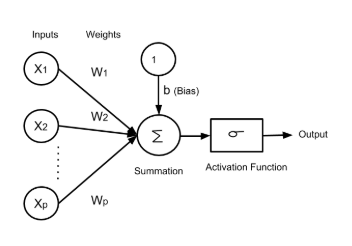
\includegraphics[width=.5\linewidth]{images/neur.png}
    \caption[Das Perceptron-Lernmodell]{Das Perceptron-Lernmodell aus \citep{Sengupta2019ATrends}}
    \label{fig:neu}
\end{figure}

\begin{comment}
\begin{xequation-} 
\centering y(x)=f(w $\circ$ x + b)
\caption[Vektorgleichung eines Neuronalen Netzes]{Vektorgleichung eines Neuronalen Netzes} 
    \label{eqn:NNN}
\end{xequation-} 

\end{comment}

\subsection{Feedforward Neural Networks}
Ein Feedforward-Neuronales Netzwerk (Vorwärts gerichtetes Netzwerk) ist ein künstliches Neuronales Netzwerk, bei dem Verbindungen zwischen den Knoten keinen Zyklus bilden. Als solches unterscheidet es sich von seinem Nachkommen: \ac{rnn}s (wiederkehrende neuronale Netze). Das vorwärtsgerichtete neuronale Netzwerk war der erste und einfachste Typ eines künstlichen neuronalen Netzwerks, das entwickelt wurde. In diesem Netzwerk bewegen sich die Informationen nur in eine Richtung vorwärts von den Eingabeknoten über die verborgenen Knoten (falls vorhanden) zu den Ausgabeknoten. Es gibt keine Zyklen oder Schleifen im Netzwerk.
\subsection{Backpropagation}
Beim maschinellen Lernen ist Backpropagation ein weit verbreiteter Algorithmus der beim Training von vorwärtsgerichteten neuronalen Netzen verwendet wird. Das Ziel eines überwachten Lernalgorithmus ist es, eine Funktion zu finden, die eine Reihe von Eingaben am besten auf ihre korrekte Ausgabe abbildet. Die Motivation für die Backpropagation besteht darin, ein mehrschichtiges neuronales Netzwerk so zu trainieren, dass es die entsprechenden internen Darstellungen lernt, ums somit eine beliebige Zuordnung von Eingabe zu Ausgabe erlernt wird. 

\subsection{Recurrent Neural Networks}
Ein \ac{rnn} ist ein spezieller \ac{nn}-Typ, der zur Verarbeitung sequentieller Daten geeignet ist. Ein wiederkehrendes neuronales Netzwerk (\ac{rnn}) ist eine Klasse künstlicher neuronaler Netzwerke, bei denen Verbindungen zwischen Knoten einen gerichteten Graphen entlang einer zeitlichen Sequenz bilden. Dies ermöglicht es, zeitlich dynamisches Verhalten zu zeigen. Von vorwärtsgerichteten neuronalen Netzen abgeleitet, können \ac{rnn}s ihren internen Zustand (Speicher) verwenden, um Sequenzen von Eingaben variabler Länge zu verarbeiten. Das Hauptmerkmal eines \ac{rnn} ist ein Zustandsvektor (in den verborgenen Einheiten), der einen Speicher aller vorherigen Elemente der Sequenz verwaltet. Eine einfache \ac{rnn} ist in der Abbildung \ref{fig:rnn} dargestellt. Wie zu sehen ist, hat ein \ac{rnn} eine Rückkopplungsverbindung, die die verborgenen Neuronen über die Zeit verbindet. Zum Zeitpunkt \textit{t} empfängt der \ac{rnn} als Eingabe das aktuelle Sequenzelement \textit{x\textsuperscript{t}} und den verborgenen Zustand aus dem vorherigen Zeitschritt \textit{h\textsuperscript{t} - 1}. Als nächstes wird der verborgene Zustand auf \textit{h\textsuperscript{t}} aktualisiert und schließlich wird die Ausgabe des Netzwerks \textit{o\textsuperscript{t}} berechnet. Auf diese Weise hängt der aktuelle Ausgang \textit{h\textsuperscript{t}} von allen vorherigen Eingängen \textit{x\textsuperscript{t}} ab.
\begin{figure}[H]
    \centering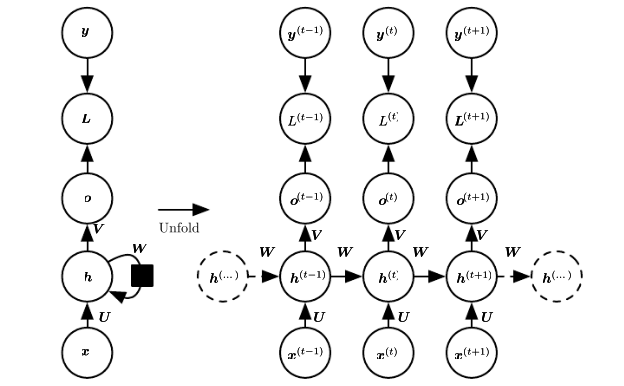
\includegraphics[width=.9\linewidth]{images/rnn.png}
    \caption[Eine Standard-RNN]{Eine Standard-RNN. Die linke Seite der Figur ist eine Standard-RNN. Der Zustandsvektor in den versteckten Einheiten wird mit \textit{s} bezeichnet. Auf der rechten Seite ist dasselbe Netzwerk zeitlich entfaltet, um darzustellen, wie der Zustand im Laufe der Zeit aufgebaut ist. \citep{IanGoodfellowYoshuaBengio2016DeepLearning}}
    \label{fig:rnn}
\end{figure}

\paragraph{Limitationen von RNNs}
Theoretisch sind \ac{rnn}s in der Lage, mit langfristigen Abhängigkeiten umzugehen. Eine der Grundidee von \ac{rnn} war es, dass sie möglicherweise Informationen die ganz vorne in einer Sequenz abgebildet werden, verwenden können, um die Sequenz zu verstehen. Manchmal müssen nur die aktuellen Informationen angesehen werde, um die vorliegende Sequenz zu verstehen. Angenommen das nächste Wort basierend auf den vorherigen soll vorhergesagt werden. Wenn versucht wird, das letzte Wort in \enquote{Die Wolken sind am Himmel...} vorherzusagen, brächte das Model keinen weiteren Kontext - es ist ziemlich offensichtlich, dass das nächste Wort \enquote{blau} sein wird. In solchen Fällen, in denen die Lücke zwischen den relevanten Informationen und dem Ort, an dem sie benötigt werden, gering ist, können \ac{rnn}s lernen, die Informationen der Vergangenheit zu verwenden. Es gibt aber auch Fälle, in denen mehr Kontext benötigt wird. Wenn das Modell versuchen soll, das letzte Wort im Satz \enquote{Ich bin in Frankreich aufgewachsen ... ich spreche fließend Französisch} vorherzusagen zum Beispiel. Es ist durchaus möglich, dass die Lücke zwischen den relevanten Informationen und dem Punkt, an dem sie benötigt werden, sehr groß wird. Leider können \ac{rnn}s mit zunehmender Lücke nicht mehr lernen, die Informationen miteinander zu verbinden.


\subsection{LSTM}
Long short-term memory (auf deutsch langes Kurzzeitgedächtnis) - normalerweise nur als \ac{lstm}s bezeichnet - sind eine spezielle Art von \ac{rnn}, mit der Langzeitabhängigkeiten gelernt werden können. Sie wurden als erstes von \citep{Hochreiter1997LongMemory} vorgestellt und von vielen Menschen in ihren folgenden Arbeiten verfeinert und populär gemacht. \ac{lstm}s wurden explizit entwickelt, um das Problem der langfristigen Abhängigkeit zu vermeiden. Das lange Erinnern an Informationen ist ihr Standardverhalten. Alle \ac{rnn}s haben die Form einer Kette sich wiederholender Module eines neuronalen Netzes. In Standard-\ac{rnn}s hat dieses sich wiederholende Modul eine sehr einfache Struktur. \ac{lstm}s haben ebenfalls diese kettenartige Struktur, aber das sich wiederholende Modul hat eine andere Struktur. Anstatt nur eine einzige neuronale Netzwerkschicht zu haben, gibt es vier, die auf ganz besondere Weise interagieren. \ac{lstm} kann Abhängigkeiten lernen, die sich über beliebig lange Zeitintervalle erstrecken. 

\paragraph{LSTM mit Forget Gates}

Bei langen, kontinuierlichen Eingaben ohne explizit markierte Start- und Endpunkte der Sequenz würde der \ac{lstm} unbegrenzt wachsen und schließlich dazu führen, dass das Netzwerk instabil wird. Das Modell würde die Zyklen oder Sequenzen aus den Daten nicht lernen. Das Modell würde nicht zurückgesetzt, wenn die nicht manuell in Sequenzen geeigneter Größe getrennt würde. Im Idealfall sollte das \ac{lstm} lernen, den Inhalt der Speicherzelle zurückzusetzen, nachdem die Verarbeitung einer Sequenz abgeschlossen ist und bevor eine neue Sequenz gestartet wird. Um dieses Problem zu lösen, wurde eine neue \ac{lstm}-Architektur mit \enquote{forget gates} eingeführt \cite{Cummins2000ArticleComputation}.

\begin{figure}[H]
    \centering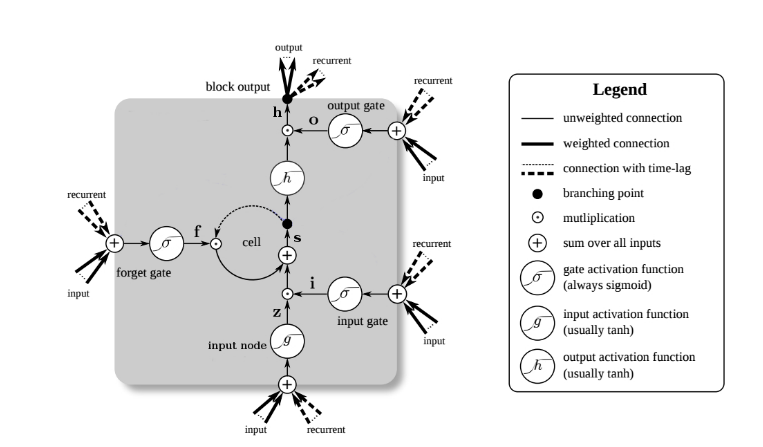
\includegraphics[width=1\linewidth]{images/lstm.png}
    \caption[Das Perceptron-Lernmodell]{Eine LSTM-Einheit mit Forget Gates in \cite{Cummins2000ArticleComputation} vorgestellt. Bild entnommen aus \citep{Greff2015TRANSACTIONSOdyssey}}
    \label{fig:lstm}
\end{figure}

Die Hauptkomponenten der \ac{lstm}-Einheit sind:

\begin{enumerate}
    \item \textbf{Input}: Die \ac{lstm}-Einheit verwendet den aktuellen Eingabevektor und die Ausgabe des vorherigen Zeitschritts (durch die wiederkehrenden Neuronen). Die gewichteten Eingaben werden summiert und durch \textit{tanh}-Aktivierung geleitet.
    \item \textbf{Input gate}: Das Input gate liest den Input, berechnet die gewichtete Summe und wendet die Sigmoidaktivierung an. Das Ergebnis wird mit \textit{z} multipliziert, um den in die Speicherzelle fließenden Eingang bereitzustellen.
    \item \textbf{Forget Gate}: Das Forget Gate ist der Mechanismus, durch den ein \ac{lstm} lernt, den Speicherinhalt zurückzusetzen, wenn er alt wird und nicht mehr relevant ist. Dies kann beispielsweise passieren, wenn das Netzwerk mit der Verarbeitung einer neuen Sequenz beginnt. Das Forget Gate liest den Input und den wiederkehrenden Teil und wendet eine Sigmoidaktivierung an. Das Ergebnis \textit{f} wird mit dem Zellenzustand im vorherigen Zeitschritt multipliziert, wodurch der Speicherinhalt vergessen werden kann, der nicht mehr benötigt wird.
    \item \textbf{Memory cell}: Der aktuelle Zellenzustand wird berechnet, indem irrelevante Informationen (falls vorhanden) aus dem vorherigen Zeitschritt vergessen und relevante Informationen (falls vorhanden) aus der aktuellen Eingabe akzeptiert werden.
    \item \textbf{Output gate}: Das Output gate nimmt die gewichtete Summe vom Input und dem wiederkehrenden Teil und wendet die Sigmoidaktivierung an, um zu steuern, welche Informationen aus der \ac{lstm}-Einheit herausfließen sollen.
    \item \textbf{Output}: Der Ausgang der \ac{lstm}-Einheit wird berechnet, indem der Zellenzustand  durch ein \textit{tanh} geleitet und mit dem Output gate multipliziert wird.
\end{enumerate}






\subsection{Encoder-Decoder Modell}
Neuronale Netze können bei einer Reihe von Aufgaben des \ac{nlp} erfolgreich eingesetzt werden und das Encoder-Decoder Modell \citep{cho2014learning} ist eines dieser Netze. Dieses Modell besteht aus zwei Blöcken. Der Codierer ist für das Codieren einer Eingabesequenz in einen festen dimensionalen Darstellungsvektor verantwortlich. Dieser Vektor wird auch \enquote{Kontextvektor} genannt. Zu den Vorteilen des Encoder-Decoder Modells gehört die Fähigkeit, Sequenzen beliebiger Länge zu einer festen Vektordarstellung zu verarbeiten. Codierer können mit verschiedenen Decodierern zum Training verbunden werden, indem die dazwischen eine codierte \textit{Darstellung} an den Decoder übergeben wird.
\begin{figure}[H]
    \centering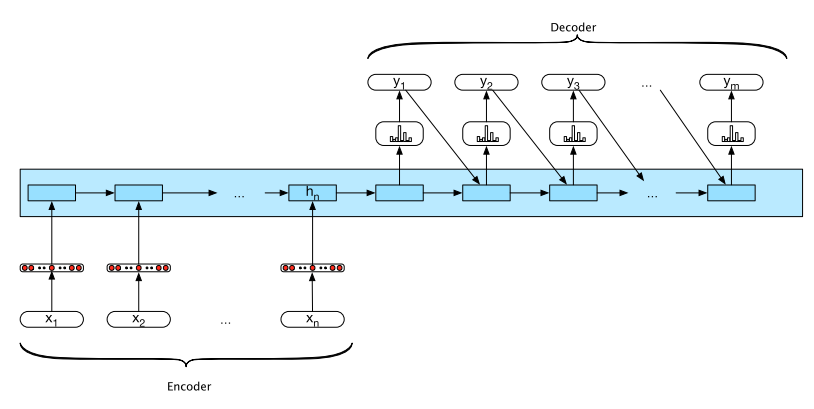
\includegraphics[width=1\linewidth]{images/dem.png}
    \caption[Encoder-Decoder Modell]{Encoder-Decoder Modell aus \citep[S. 194]{Jurafsky2014SpeechProcessing}}
    \label{fig:dem}
\end{figure}

Die Elemente des Netzwerks auf der linken Seite verarbeiten die Eingabesequenz und sind somit für das encoden verantwortlich. Der gesamte Zweck des Encoders besteht darin, eine kontextualisierte Darstellung der Eingabe zu erzeugen. Diese Darstellung wird beim letzten verborgenen Zustand $h_{n$} verkörpert.
Das Decoder Netzwerk auf der rechten Seite nimmt diesen Zustand von $h_{n$} an und erzeugt autoregressiv eine Folge von Ausgängen. 









%%%%%%%%%%%%%%%%%%%%%%%%%%%%%%%%%%%%%%%%%%%%%%%%%%%%%%%%%%%%%%%%%%%%%%
\section{Natural Language Processing}

Verarbeitung natürlicher Sprache, das Natutal Language Processing (\ac{nlp}), ist eine theoretisch motivierte Reihe von Computertechniken, für die automatische Analyse und Darstellung der menschlichen Sprache \citep[S. 48]{cambria2014jumping}. Die Verarbeitung natürlicher Sprache (\ac{nlp}) zielt darauf ab, Text zu lesen oder der Sprache zu hören und daraus aussagekräftige Informationen zu extrahieren. 

\subsection{Sprachmodelle}
Ein Sprachmodell bildet die Beziehungen der Wörter durch die Eigenschaften der Sprache ab. Anstatt sie mit Regeln zu beschreiben, was zu komplex wäre, nutzt ein Sprachmodell die Wahrscheinlichkeitsrechnung. Dadurch ist es in der Lage, das Wort vorherzusagen, das bei einer bestimmten Folge von Wörtern folgen wird. In ausgebauten Modellen wird mehr der Kontext berücksichtigt, von Sequenzen vorheriger Wörter bis hin zu Sätzen, Absätzen oder ganzen Dokumenten. Man kann ein Sprachmodell verwenden, um den Fortgang eines Satzes vorherzusagen, aber auch um neue Sätze zu erzeugen \citep{goodman2001bit}.

\paragraph{N-Gram Modelle}
Ein Beispiel für ein Sprachmodell ist das N-Gram-Modell. Ein N-Gramm ist ein N-Zeichen-Slice einer längeren Zeichenfolge \citep{cavnar1994n}. N-Gram-Sprachmodelle sind einfache Modelle, die durch Wortfolgen der Länge N definiert sind. Wenn N = 1 ist, wird es als \enquote{Unigram} bezeichnet, wenn N = 2 als \enquote{Bigram}. Es wird jedes Wort als Einheit genommen und seine Wahrscheinlichkeit berechnet. Dies geschieht, indem sein Auftreten im Dokument gezählt und durch die Gesamtzahl der Wörter dividiert wird. 


\subsection{Vektoren zur Darstellung der Bedeutung von Wörtern}
Wörter, die in ähnlichen Kontexten vorkommen, haben tendenziell ähnliche Bedeutungen. Nach Ludwig Wittgenstein ist die Bedeutung eines Wortes, seine Nutzung in der Sprache \citep{wittgenstein2009philosophical}. Wörter können als Vektoren dargetsellt und somit die Bedeutung im Allgemeinen auf einer Koexistenzmatrix, dargestellt werden. Sprachmodelle sind statistische Modelle, sie erfordern daher quantifizierbare und kontinuierliche Darstellungen. Aber Wörter sind andererseits diskrete Einheiten. Ein einfacher Ansatz, um sie auf quantifizierbare Weise darzustellen, besteht darin, die Merkmale mit einem Vektor zu codieren und für jedes Wortmerkmal seine Position auf binäre Weise zu identifizieren. Dieses wird als \textit{One-Hot-Vektor} bezeichnet. Die Einfachheit wird durch die hohe Dimension dieser Vektoren und die damit verbundene Komplexität überschattet. Um dieser Einschränkung zu entgehen, kommt das Encoder-Decoder-Modell ins Spiel und wird verwendet, um eine Darstellung mit reduzierter Dimensionalität zu codieren. Ein Textkorpus kann dann in numerische Vektoren codiert werden, die auch als \textit{word embeddings} oder auf Deutsch \textit{Worteinbettungen} bekannt sind. Sobald Wörter codiert sind, entsteht ein sog. \textit{Vektor Raum Modell (VSM)}. Dadurch kann einfache lineare Algebra angewendet werden, welches die Berechnung der Beziehung zwischen Wörtern ermöglicht. Folgendes Beispiel aus \citep[S. 105]{Jurafsky2014SpeechProcessing} soll darstellen wie so eine Vektorisierung der Wörter und somit der Gewinn an Bedeutung erfolgt:

 \paragraph{Textausschnitt}
 \textit{...is traditionally followed by \textbf{cherry} pie, a traditonal desert often mixed, such as \textbf{strawberry} rhubarb pie. Apple pie computer peripherals and personal \textbf{digital} assistants. These devices usually a computer. This includes \textbf{information} available on the internet...}




    
\begin{figure}[H]
    \centering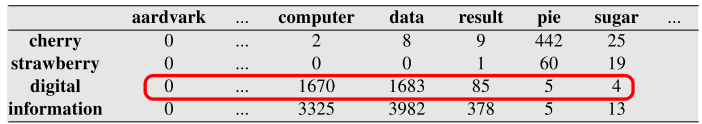
\includegraphics[width=0.6\linewidth]{images/mat.png}
    \caption[Wort-Wort-Matrix]{Wort-Wort-Matrix aus \citep[S. 105]{Jurafsky2014SpeechProcessing}}
    \label{fig:mat}
\end{figure}

\begin{figure}[H]
    \centering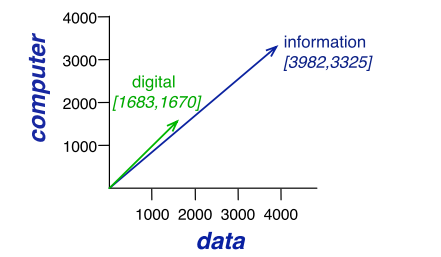
\includegraphics[width=0.5\linewidth]{images/vec.png}
    \caption[Visualisierung von Wortvektoren]{Visualisierung von Wortvektoren aus \citep[S. 105]{Jurafsky2014SpeechProcessing}}
    \label{fig:vec}
\end{figure}



In Abbildung \ref{fig:mat} ist zu sehen, wie sich aus dem vorherigen Beispiel eine Wort-Wort-Matrix bildet. Diese Matrix gibt den vorhanden Wörtern des darzustellenden Fensters untereinander eine Bedeutung. Diese Bedeutung wird in der Abbildung \ref{fig:vec} dargestellt.

\subsection{Kosinus-Ähnlichkeit}
Um die Ähnlichkeit zwischen zwei Vektoren V und W darzustellen, also die Vektorähnlichkeit anzugeben, kann die Kosinus-Ähnlichkeit verwendet werden.

\begin{xequation-} 
\centering \cos(v, w) = {\mathbf{v} \cdot \mathbf{w} \over \|\mathbf{v}\| \|\mathbf{w}\|} = \frac{ \sum_{i=1}^{n}{v_i \cdot w_i} }{ \sqrt{\sum_{i=1}^{n}{(v_i)^2}} \cdot \sqrt{\sum_{i=1}^{n}{(w_i)^2}} }
\caption[Kosinus-Ähnlichkeit]{Kosinus-Ähnlichkeit} 
    \label{eqn:KSA}
\end{xequation-} 

Mit den zu analysierenden 4 Wörtern \enquote{pie}, \enquote{data}, \enquote{computer} und \enquote{information} kann durch die Kosinus-Ähnlichkeit bestimmt werden, welches der Wörter eine Ähnlichkeit untereinander aufweist. Das Wort \enquote{cherry} hat weniger mit \enquote{information} gemeinsam, als \enquote{digital} mit \enquote{information}. Da diese Wörter in einem geringeren Kontext auftauchen \citep[S. 105]{Jurafsky2014SpeechProcessing}.

\begin{table}[H]
{\small
    \begin{tabularx}{\textwidth}{X X X X} 
\hline     
                  &\textbf{pie}  & \textbf{data} & \textbf{computer}  \\ 
\hline    
    \textbf{cherry}      & 442        & 8 & 2         \\ 
    \textbf{digital}   & 5        & 1683 & 1670          \\ 
    \textbf{information} & 5        & 3982 & 3325           \\ 
    \end{tabularx}
\caption{Wort-Wort-Matrix}
    \label{tab:cos}
}
\end{table}



Auf der Tabelle \ref{tab:cos} wird die Formel angewendet und dadurch ergibt sich das Ergebnis, welches zeigt, dass die beiden Wörter \enquote{digital} und \enquote{information} eine relativ ähnliche Bedeutung haben und die Wörter \enquote{cherry} und \enquote{information} eine niedrige. 


\begin{xequation-} 
\centering cos(cherry, information) = $\frac{442\ast 5+8\ast3982+2\ast3325}{\sqrt{442^{2} +8^{2} +2^{2}}\ast \sqrt{5^{2} +3982^{2} +3325^{2}}}$ = 0.17
\newline
\newline
\centering cos(digital, information) = $\frac{5\ast 5+1683\ast3982+1670\ast3325}{\sqrt{5^{2} +1683^{2} +1670^{2}}\ast \sqrt{5^{2} +3982^{2} +3325^{2}}}$ = 0.996 
\end{xequation-} 




\subsection{Word2Vec}
In \citep{mikolov2013efficient} wird das Word2vec dargestellt.
Word2vec ist eine Gruppe verwandter Modelle, mit denen Worteinbettungen erstellt werden. Diese Modelle sind flache, zweischichtige neuronale Netze, die darauf trainiert sind, sprachliche Kontexte von Wörtern zu rekonstruieren. Word2vec verwendet als Eingabe einen großen Textkorpus und erzeugt einen Vektorraum, der typischerweise mehrere hundert Dimensionen umfasst, wobei jedem eindeutigen Wort im Korpus ein entsprechender Vektor im Raum zugewiesen wird. Wortvektoren werden im Vektorraum so positioniert, dass Wörter, die gemeinsame Kontexte im Korpus haben, im Raum nahe beieinander liegen. Word2vec wurde 2013 von einem Forscherteam unter der Leitung von Tomas Mikolov bei Google erstellt und veröffentlicht. Wörter in ähnlichen Kontexten haben ähnliche Bedeutungen. Intuitiv bedeutet dies, dass Wörter, die viele Kontexte gemeinsam haben, einander ähnlich sind \citep{goldberg2014word2vec}. 










%%%%%%%%%%%%%%%%%%%%%%%%%%%%%%%%%%%%%%%%%%%%%%%%%%%%%%%%%%%%%%%%%%%%%%










%DONE%%%%DONE%%%%DONE%%%%DONE%%%%DONE%%%%DONE%%%%DONE%%%%DONE%%%%DONE%
%%%%%%%%%%%%%%%%%%%%%%%%%%%%%%%%%%%%%%%%%%%%%%%%%%%%%%%%%%%%%%%%%%%%%%    
\chapter{Question Answering - Literaturstudie} 
%%%%%%%%%%%%%%%%%%%%%%%%%%%%%%%%%%%%%%%%%%%%%%%%%%%%%%%%%%%%%%%%%%%%%%


    
Mit Suchmaschinen wird es den Benutzern immer leichter an gewünschte Informationen heranzukommen. Da Benutzer Schwierigkeiten haben, sich in der Fülle an Informationen der jetzt verfügbaren Online-Informationen zurechtzufinden, wird die Notwendigkeit automatisierter Systeme zur Beantwortung von Fragen immer dringlicher. Es erde Systeme nötig, mit denen ein Benutzer eine Frage in der Alltagssprache stellen und schnell und präzise eine Antwort erhalten kann und mit ausreichendem Kontext. In der Vergangenheit konnten Suchmaschinen noch nicht wirklich Fragen beantworten, sonder lieferten Ranglisten von Dokumenten zurück. Diese Dokumente liefern dem Benutzer jedoch nicht immer die gewünschten Antworten \citep[S. 275]{Hirschman2001NaturalHere}. In Abbildung \ref{fig:google} ist zu sehen, wie moderne Suchmaschinen Question Answering anbieten.

\begin{figure}[H]
    \centering
\includegraphics[width=1\linewidth]{images/google.png}
    \caption[Question Answering mit Google]{Question Answering mit Google}
    \label{fig:google}
\end{figure}


\section{Definitionen der Begriffe}
Um das Question Answering zu verstehen, werden zunächst die zugehörigen Begriffe definiert. Um eine Frage zu beantworten, muss ein Question Answering System die Frage analysieren, möglicherweise im Zusammenhang mit einer laufenden Interaktion. Es muss eine oder mehrere Antworten finden, indem es Online-Ressourcen konsultiert und es muss dem Benutzer die Antwort in einer geeigneten Form präsentieren, möglicherweise verbunden mit Begründung oder unterstützendem Material \citep[S. 276]{Hirschman2001NaturalHere}. 

\textbf{Question Answering Systeme} sind Sytsteme, die duch Informationsabruf automatisch Antworten zur gestellten Frage generieren, die Menschen in ihrer natürlichen Sprache stellen. Entweder mithilfe einer vorstrukturierten Datenbank oder einer Sammlung von Dokumenten in natürlicher Sprache \citep{Chali2011ImprovingKernels}\citep{Dwivedi2013ResearchSystem}\citep{Ansari2016IntelligentNetwork}\citep{Lende2016QuestionTechniques}. Es wird dabei abgegrenzt, zwischen \textbf{Fragensatz}, also der gestellten Frage und dem \textbf{Fragentyp}, welches den Zweck einer Kategorisierung der Frage ausweist. In der Literatur bezieht sich der Begriff \textbf{Antworttyp} auf eine Klasse von Objekten, nach denen die Frage sucht. \textbf{Fragenfokus} ist die Eigenschaft oder Entität, nach der die Frage sucht. \textbf{Fragethema} ist das Objekt oder Ereignis, um das es in der Frage geht \citep[S. 2]{CalijorneSoares2018ASystems}. Eine Textpassage welches ein Kandidat für eine Frage ist, wird \textbf{Kandidatenantwort} genannt und ist der Text, der nach seiner Eignung als Antwort eingestuft wird \citep{RetrievalOpen-DomainQuestion-Answering}.

Fragen können nach \textbf{Antworttyp} unterschieden werden: sachliche Antworten vs. Meinung vs. Zusammenfassungen. Obwohl das Verständnis beispielsweise häufig andere Arten von Fragen enthält (Worum geht es in dieser Geschichte? oder Wie steht der Autor zur Hauptfigur in dieser Geschichte?) konzentriert sich das Question Answering meistens auf Fragen mit sachlichen Antworten. Als nächstes können Fragen nach der \textbf{Fragenart} unterscheiden werden: \enquote{Ja / Nein-Fragen}, \enquote{w-Fragen} (Wer war der erste Präsident? Wie viel wiegt ein Wal?), \enquote{indirekte Abfragen} (Liste alle ... auf!) und \enquote{Befehle} (Nennen Sie alle Präsidenten ...). Einige Arten von Fragen sind schwieriger als andere zu beantworten. Zum Beispiel, \enquote{Warum- und Wie-Fragen}, weil sie das Verständnis von Kausalität oder Beziehungen erfordern und diese typischerweise als separate Nebensätze ausgedrückt werden. Die Antworten können lang oder kurz sein, sie können Listen oder Erzählungen sein. Sie können je nach Verwendungszweck variieren. Wenn ein Benutzer beispielsweise eine Begründung wünscht, erfordert dies eine längere Antwort. Es gibt auch verschiedene Methoden zum Erstellen einer Antwort: durch Extrahieren, also das Ausschneiden und Einfügen von Ausschnitten aus den Originaldokumenten, die die Antwort enthalten, oder durch Generieren von neuem Text \citep [S. 277-278]{Hirschman2001NaturalHere}. 

Grundsätzlich wird zwischen Faktoiden-, Listen-, Definitions- und komplexe Fragen unterschieden \citep{Kolomiyets2011APerspective}. \textbf{Faktoide Fragen} sind diejenigen, die nach einer einfachen Tatsache fragen und mit wenigen Worten beantwortet werden können, (zum Beispiel: Wie weit ist es von der Erde zum Mars?). \textbf{Liste Fragen} fordern als Antwort eine Reihe von Entitäten, die ein bestimmtes Kriterium erfüllen (zum Beispiel: Wann hat Brasilien Fußball Weltmeisterschaften gewonnen?) \citep{Heie2012QuestionModelling}. \textbf{Definitionsfragen} erwarten im Gegenzug eine Zusammenfassung oder eine kurze Passage (zum Beispiel: Wie funktioniert die Mitose einer Zelle?) \citep{Neves2015QuestionBiology}. Im Gegensatz dazu handelt es sich bei den \textbf{komplexen Fragen} um Informationen in einem Kontext. Normalerweise ist die Antwort eine Zusammenführung von abgerufenen Passagen.


\section{Systemarchitektur des Question Answerings} %2 Seiten

%%%%%%%%%%%%%%%%%%%%%%%%%%%%%%%%%%%%%%%%%%%%%%%%%%%%%%%%%%%%%%%%%%%%%%    
% TODO
%    %write more []
%
%%%%%%%%%%%%%%%%%%%%%%%%%%%%%%%%%%%%%%%%%%%%%%%%%%%%%%%%%%%%%%%%%%%%%%    

Allgemein lässt sich ein Question Answering System in 3 Module unterteilen (siehe Abbildung \ref{fig:architektur}):
\begin{itemize}
    \item \textbf{Analyse der Frage}
    \item \textbf{Auswahl geeigneter Dokumente}
    \item \textbf{Verarbeitung der Antwort} 
\end{itemize}

Der Prozess des Question Answerings geht vom Benutzer aus und das System erhält vom Benutzer eine Eingabe, eine Frage, welches in natürlicher Sprache gestellt wird. Das System soll diese Frage verstehen und dafür findet eine \textbf{Analyse der Frage} statt. Die Analyse besteht darin, die Art der Frage herauszufinden, also den Schwerpunkt der Frage oder die Intention zu verstehen \citep{Malik2013DomainSystem}. Die Analyse der vom Nutzer gestellten Fragen wird in zwei Verfahren unterteilt. Das erste Verfahren beschäftigt sich mit der Struktur der Frage, das zweite Verfahren, die Frage so zu transformieren, das Sie mit der \ac{qa}-Domäne kompatibel ist \citep{Hamed2016AClassification}.

Anders als bei der Analyse der gestellten Frage, wird bei der \textbf{Auswahl geeigneter Dokumente} eine Reihe relevanter Dokumente selektiert. Diese dienen als Mögliche Kandidaten für die beantwortung der Frage \cite{Malik2013DomainSystem}. Die abgerufenen Daten können nach ihrer Relevanz für die Frage eingestuft werden \citep{Neves2015QuestionBiology}. 

Die \textbf{Verarbeitung der Antwort} ist die schwierigste Aufgabe beim Question Answering. Dieses Modul verwendet Extraktionstechniken. Diese Techniken sollen aus den Dokumenten, die als Kandidaten dienen, eine Antwort präsentieren \citep{Bhoir2014QuestionApproach}. Die Antwort muss eine einfache Antwort auf die Frage sein, es kann jedoch erforderlich sein, Informationen aus verschiedenen Quellen zusammenzuführen.

\begin{figure}[H]
    \centering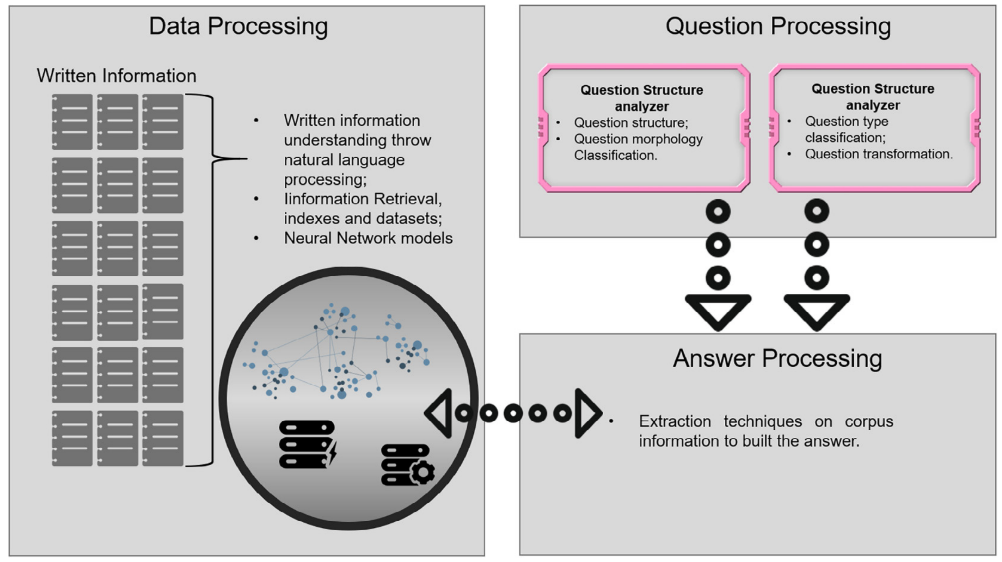
\includegraphics[width=1\linewidth]{images/arch.png}
    \caption[Allgemeine Systemarchitektur mit 3 Hauptmodulen]{Allgemeine Systemarchitektur mit 3 Hauptmodulen \cite [S. 3]{CalijorneSoares2018ASystems}}
    \label{fig:architektur}
\end{figure}
\section{Geschichte des Question Answerings}

%%%%%%%%%%%%%%%%%%%%%%%%%%%%%%%%%%%%%%%%%%%%%%%%%%%%%%%%%%%%%%%%%%%%%%    
% TODO
%    %graphs []
%
%%%%%%%%%%%%%%%%%%%%%%%%%%%%%%%%%%%%%%%%%%%%%%%%%%%%%%%%%%%%%%%%%%%%%%    

Tatsächlich geht die Geschichte des Question Answering bis in die 60'er Jahre zuruck. Mit \citep{Simmons1964IndexingQuestions} wurde im Jahr 1965 versucht, englische Fragen mittels eines Computers zu beantworten. Mit \textbf{BASEBALL} \citep{Green1961Baseball:Question-answerer} wurden bereits im Jahr 1961 Baseball-Spiele analysiert. Während BASEBALL selbst nach aktuellen Maßstäben im Umgang mit der Syntax und Semantik von Fragen relativ hoch entwickelt war, war es in Bezug auf seine Domäne - nur Baseball - und durch die Tatsache, dass es in erster Linie als Schnittstelle zu einer strukturierten Datenbank gedacht war, begrenzt und nicht als Schnittstelle zu einer großen Textsammlung gedacht. In dieser Hinsicht war BASEBALL als „Frontends für Datenbanken in natürlicher Sprache“ konzipiert wurden. Anstatt Benutzer dazu zu zwingen, die Struktur einer Datenbank und eine spezielle Sprache für deren Abfrage zu lernen, bestand das Ziel darin, die Kommunikation in ihrer eigenen Sprache mit einer Schnittstelle zu ermöglichen. Das Frontend konnte dann die Sprache verstehen und diese in eine Datenbankabfrage umwandeln \citep[S. 279-280]{Hirschman2001NaturalHere}.

Das bekannteste andere frühe Werk ist das \textbf{LUNAR}-System. LUNAR wurde entwickelt, \enquote{um einem Mondgeologen einen bequemen Zugriff auf die chemischen Analysedaten, die sich infolge der Apollo-Mondmission angesammelt haben zur Mondgesteins- und Bodenzusammensetzung zu ermöglichen, diese zu vergleichen und auszuwerten} \citep{4-8ProgressGeology}. LUNAR könnte Fragen beantworten wie \enquote{Wie hoch ist die durchschnittliche Aluminiumkonzentration in Gesteinen mit hohem Alkaligehalt?} oder \enquote{Wie viele Brescias enthalten Olivin?}. Es war mehr als ein Spielzeug und wurde 1971 auf einer Mondwissenschaftskonvention demonstriert und konnte 90\% der von arbeitenden Geologen gestellten Fragen ohne vorherige Anweisung zur Formulierung beantworten \citep[S. 280]{Hirschman2001NaturalHere}. 


In den 1980er und 1990er Jahren wurden Wissensbasierte Systeme, die normalerweise nur für beschränkte Anwendungsbereiche entwickelt wurden, sehr beliebt. Wissensbasierte Systeme  eignen sich gut für ein Framework zur Beantwortung von Fragen, bei dem der Benutzer mit einem bestimmten Problem konfrontiert wird. Der Zugriff auf die Wissensdatenbank erfolgt normalerweise über Menüs oder eine Schnittstelle in natürlicher Sprache. Das System selbst stellt dem Benutzer interaktiv zusätzliche Fragen, um die Absicht des Benutzers besser zu verstehen. Um das Problem zu lösen, verwendet das System das in der Wissensdatenbank verfügbare Wissen und die vom Benutzer bereitgestellten zusätzlichen Informationen \citep [S. 5415]{Kolomiyets2011APerspective}. Bekannte Beispiele sind das \textbf{MYCIN-System} \citep{edward1976shortliffe}, welches als Enzyklopädie für medizinische Konzepte Antworten geben sollte und das \textbf{SHRDLU-System} \citep{winograd1971procedures} welches durch sein Sprachverständnis Roboter steurte und somit Spielzeugblöcke bewegen konnte.

Die Ära des zeitgenössischen Question Answerings begann 1999 mit der aufnahme des Question Answerings in das Wettbewerbspfad von \textbf{TREC-9} (\enquote{The ninth Text REtrieval Conference}), welches eine  Konferez ist, die die Forschung für das Information Retrieval fördern soll. In dieser Konforenz wurde eine Herausforderung für das Question Answering definiert, welches darin bestand, angesichts einer großen Sammlung von Textdokumenten eine präzise Antwort auf eine Frage in natürlicher Sprache zu geben \citep{VoorheesReportTREC-9}. \ac{trec} hatte einen großen Einfluss auf das Interesse am Question Answering und auf die Entwicklung von Bewertungsmaßnahmen, mit denen die Leistung von Systemen verglichen wird \citep{voorhees2005trec}. 


\section{Klassifizierung der QA-Systeme}
\subsection{Klassifizierung nach der Domäne}
%%%%%%%%%%%%%%%%%%%%%%%%%%%%%%%%%%%%%%%%%%%%%%%%%%%%%%%%%%%%%%%%%%%%%%    
% TODO
%   % Tabelle mit den Arten
%%%%%%%%%%%%%%%%%%%%%%%%%%%%%%%%%%%%%%%%%%%%%%%%%%%%%%%%%%%%%%%%%%%%%%    
Im Allgemeinen kann das Question Answering in Open-Domain Question Answering und Closed-Domain Question Answering unterteilt werden. Die Beantwortung von Fragen zu geschlossenen Domänen befasst sich mit Fragen unter einer bestimmten Domäne und kann als einfachere Aufgabe angesehen werden, da \ac{nlp}-Systeme domänenspezifisches Wissen nutzen können, das häufig in Ontologien formalisiert wird. Alternativ kann sich eine geschlossene Domäne auf eine Situation beziehen, in der nur eine begrenzte Art von Fragen akzeptiert wird, z. B. Fragen, die eher beschreibende als prozedurale Informationen erfordern. Die Beantwortung von Fragen in offenen Domänen behandelt Fragen zu fast Allem und kann sich nur auf allgemeine Ontologien wie \enquote{DBpedia} stützen \citep{Mervin2013AnSystem}. Einen Vergleich der Systeme kann aus der Tabelle \ref{tab:tab1} entnommen werden.

\textbf{Open Domain Question Answering} Systeme sind nicht auf eine bestimmte Domain beschränkt und bieten eine kurze Antwort auf eine Frage in natürlicher Sprache. Das Web ist die beste Quelle, um Informationen zu erhalten, da das Internet in großem Umfang genutzt wird, und die meisten webbasierten Systeme zur Beantwortung von Fragen funktionieren für offene Domänen \citep{yogish2016survey}. Das Open-Domain-\ac{qa}-System hängt von Informationen wie dem World Wide Web und der universellen Ontologie ab und kann fast Alles beantworten \citep{SreelakshmiOPENLABELING}. Open Domain \ac{qa}-Systeme wenden ein allgemeines Vokabular an und erfordern kein domänenspezifisches Vokabular. Benutzer benötigen keine domänenspezifischen Kenntnisse, um Fragen vorzubereiten. Open Domain \ac{qa}-Systeme bestehen aus einem großen \enquote{Repository} von Fragen und suchen im Allgemeinen nach Antworten in einer großen Dokumentensammlung. In Open Domain \ac{qa}-Systemen kann Wikipedia als Informationsquelle verwendet werden. In Open-Domain \ac{qa}-Systemen ist die Qualität der Antworten, die von Benutzern generiert werden, gering. Open Domain \ac{qa}-Systeme sind domänenunabhängig und hängen von Weltdaten und der grundlegenden Ontologie ab \citep{biswas2014framework}. Im Open Domain \ac{qa}-System gibt es keine Einschränkung der Domain. Open-Domain \ac{qa}-Systeme eignen sich eher für eine große Anzahl von Gelegenheitsbenutzern \citep[S. 20]{ChandraASystem}.

In \textbf{Closed Domain Question Answering} Systemen gibt es eine Einschränkung der Domäne, die beantwortung der Fragen ist verbunden an eine bestimmte Domäne. Das System besteht aus einem begrenzten \enquote{Repository} domänenspezifischer Fragen und kann eine begrenzte Anzahl von Fragen beantworten. Daher ist in \ac{qa}-Systemen mit geschlossenen Domänen die Qualität der Antworten hoch. \ac{qa}-Systeme für geschlossene Domänen beantworten domänenspezifische Fragen, und Antworten werden in domänenspezifischen Dokumentensammlungen gesucht. \ac{qa}-Systeme mit geschlossenen Domänen sind so konzipiert, dass sie Antworten aus strukturierten Daten (z. B. Datenbanken), unstrukturierten Daten (Freitexte) und halbstrukturierten Daten (z. B. XML-kommentierten Texten) erhalten. \ac{qa}-Systeme für geschlossene Domänen verwenden domänenspezifische Terminologie und Ontologie. \ac{qa}-Systeme mit geschlossener Domäne mit begrenzter Arbeitsdomäne sind nützlicher für Benutzer, die spezielle Antworten benötigen \citep[S. 20]{ChandraASystem}.

\begin{table}[H]
{\small
    \begin{tabularx}{\textwidth}{X|X|X} 
    
                  &\textbf{Open Domain QA}  & \textbf{Closed Domain QA}  \\ 
\hline    
    \textbf{Domäne}      & unbeschränkt        & beschränkt         \\ 
    \textbf{Quelle}   & Web        & Datenbanken          \\ 
    \textbf{Qualität} & gering        & gut           \\ 
    \textbf{Nutzer} & Gelegenheitsnutzer        & Domänenexperten           \\ 
    \end{tabularx}
\caption{Vergleich des Open-Domain und Closed-Domain Question Answerings}
    \label{tab:tab1}
}
\end{table}


\subsection{Klassifizierung nach dem Fragetyp}

Neben der Domäne, werdem Question Answering Systeme nach Fragetypen klassifiziert. Diese Fragentypen sind \citep[S. 20-21]{ChandraASystem}:

\begin{itemize}
    \item \textbf{Faktoide Fragen} 
    Die faktoiden Fragen beginnen gewöhnlich mit einem W-Wort (\enquote{Was?}, \enquote{Wann?}, \enquote{Wer?}, \enquote{Wie?}). Diese Fragen sind einfach zu beantworten und basieren auf Fakten. Sie müssen in einem einzigen Satz oder einer kurzen Phrase beantwortet werden. Zum Beispiel die faktoide Frage \enquote{Was ist die Hauptstadt von Indien?} fragt nach einem Städtenamen und es ist einfach. Die Antworttypen für faktoide Fragen werden im Allgemeinen als Entitäten bezeichnet \citep{khillare2014comparative}. Fragen vom Typ Faktoid ergeben eine zufriedenstellende Antwortleistung. Im Allgemeinen sind Fragen vom Typ Faktoid ein großes Repository von Fragen. Fragen vom Typ Faktoid erfordern keine komplexe Verarbeitung natürlicher Sprache, um Antworten zu erhalten. Die Identifizierung von Fragen vom Typ Faktoid und ihre Unterklassifizierung ist eines der Forschungsprobleme im Fragebeantwortungssystem. Fragen vom Typ Faktoid können mit kurzen Sätzen wie Organisationen, Personen, Daten und Orten beantwortet werden.
    \item \textbf{Listen Fragen}
    Die Fragen nach Listen benötigen eine Liste von Fakten oder Entitäten als Antworten, z.B, listen sie die Namen der Filme im Jahr 2017 auf. Bei diesen Fragen werden die Antworttypen als Entitäten bezeichnet. Daher können die Antworten auf Listenfragen eine gute Genauigkeit ergeben. \ac{qa}-Systeme die solche Fragen beantworten benötigen keine tiefgreifende Verarbeitung natürlicher Sprache, um Antworten abzurufen. Die Techniken, die bei Fragen vom Typ Faktoid angewendet werden, eignen sich gut für Fragen vom Listentyp \citep{wu2015leveraging}.
    \item \textbf{Bestätigungsfragen} 
    Bestätigungsfragen benötigen Antworten in Form von \enquote{Ja} oder \enquote{Nein}. Zum Beispiel die Bestätigungsfrage \enquote{Ist Jesus Christus Gott und Mensch?}, fragt nach der Antwort Ja oder Nein. Zur Beantwortung von Bestätigungsfragen sind Weltwissen, Inferenzmechanismen und logisches Denken erforderlich. Einer der Vorteile von Fragen vom Typ Bestätigung, die in \ac{qa}-Systemen gestellt werden, besteht darin, dass einige erfahrene Benutzer möglicherweise nach Informationen suchen möchten, die für neues Wissen logisches Denken und Weltwissen erfordern \citep{tanwar2014effective}. Die Nachteile von Bestätigungsfragen, die in \ac{qa}-Systemen gestellt werden, bestehen darin, dass sie ein höheres Maß an Techniken zum Erwerb und Abrufen von Wissen benötigen. Abgesehen von den oben genannten Fragen zum Bestätigungstyp können Meinungsfragen erforderlich sein. \ac{qa}-Systeme verwenden Social, Web- und Opinion Mining-Techniken, um Antworten auf die Fragen vom Typ \enquote{Meinung} zu erhalten. Die Vorteile von Meinungsfragen sind, dass Meinungsdatenquellen öffentliche Meinungen enthalten, die den Benutzern bei der Beurteilung der Produkte helfen können. Die Nachteile von Fragen vom Typ Meinung sind die Erkennung von Spam oder gefälschten Inhalten in Textsystemen, was zu Problemen beim echten Argument-Mining des Textes führt.
    \item \textbf{Kausale Fragen} 
    Die Antworten auf kausale Fragen werden \enquote{nicht als faktoide Fragen} bezeichnet. Kausale Fragen benötigen Antworten auf Beschreibungen einer Entität und können mit \enquote{Warum?} oder \enquote{Wie?} beantwortet werden. Kausale Fragen werden von Benutzern gestellt, die Antworten als Gründe, Erklärungen, Ausarbeitungen usw. in Bezug auf bestimmte Objekte oder Ereignisse wünschen.
    z. B. Warum hält Professor Y eine Rede im Auditorium?
    \item \textbf{Hypothetische Fragen}
    Bei hypothetischen Fragen werden Informationen angefordert, die sich auf ein hypothetisches Ereignis beziehen und nicht spezifisch sind. Hypothetische Fragen beginnen normalerweise mit \enquote{Was würde passieren, wenn?}. Die Zuverlässigkeit und Genauigkeit dieser Fragen ist gering und hängt von den Benutzern und dem Kontext ab.
    \item \textbf{Komplexe Fragen}
    Um komplexe Fragen wie \enquote{Was sind die Gründe für Luftverschmutzung?} beantworten zu können, müssen oft Informationen aus mehreren Dokumenten abgeleitet und synthetisiert werden. Zur Beantwortung komplexer Fragen sind komplexe Verfahren erforderlich. Komplexe Fragen erfordern mehrere unterschiedliche Arten von Informationen, und es ist schwierig, Antworten zu finden. Nach \citep{basuki2016statistical} besteht eine komplexe Frage aus mehreren unabhängigen Fragen, und jede Frage sucht nach einer Antwort aus mehreren Dokumenten.
    
\end{itemize}


\subsection{Klassifizierung nach der Datenquelle}
Neben der Hauptarchitektur können \ac{qa}-Systeme nach der herkunft Ihrer Daten klassifiziert werden. In \citep{Jurafsky2014SpeechProcessing} wird das \ac{qa} unterteilt in Information Retrieval \ac{qa},  wissensbasiertes \ac{qa} und hybrides \ac{qa} \citep{Ojokoh2019ASystems}:


%%%%%%%%%%%%%%%%%%%%%%%%%%%%%%%%%%%%%%%%%%%%%%%%%%%%%%%%%%%%%%%%%%%%%%
%n-gram pattern extraction -- NLP!!
%%%%%%%%%%%%%%%%%%%%%%%%%%%%%%%%%%%%%%%%%%%%%%%%%%%%%%%%%%%%%%%%%%%%%%

\begin{itemize}
    \item \textbf{Information Retrieval QA} Basiert auf einer sehr großen Menge von Informationen, die im Web als Text oder in Ontologien vorhanden sind. Diese Art von \ac{qa} bietet eine Antwort auf die Fragen des Benutzers, indem es Textausschnitten aus dem Web oder Korpora abruft. Eine faktoide Abfrage lautet z.B.: \enquote{Wer ist der Präsident von Nigeria?}. Die Antwort lautet \enquote{Präsident Buhari im Urlaub in London}. IR-Methoden extrahieren Passagen direkt aus den passenden Dokumenten, welches sie von der gestellten Frage ableiten. Zunächst verarbeitet diese Methode die Abfrage vor, um den Antworttyp (Person, Ort oder Zeit) zu ermitteln. Die Genauigkeit der Fragenklassifizierung ist für faktoide Fragen mit benannten Entitäten als erwartete Ausgabe relativ hoch, aber Fragetypen wie Bestätigungsfragen, kausale Fragen, hypothetische Fragen oder komplexe Fragen können viel schwieriger sein, da sie ein tiefes Verständnis der Abfrage erfordern. Anschließend werden Abfragen für die Suche erstellt, um Suchmaschinen abzufragen. Dies beinhaltet das Isolieren von Begriffen aus der Frage, die eine Abfrage bilden, die dann an ein Abrufsystem gestellt werden. Dies beinhaltet gelegentlich das Entfernen von Stoppwörtern und Satzzeichen. Als nächstes müssen die von der Suchmaschine gelieferten Dokumente oder Passagen geordnet werden. Dieses Ordnen der Dokumente kann z.B. mit der Methode \enquote{tf-idf}, einer Relevanzmodellierungsansatz für die Bewertung von Passagen oder Dokumenten ausgeführt werden \citep[S. 467 - 470]{Jurafsky2014SpeechProcessing}.
    Zuletzt werden potenzielle Zeichenfolgen für die Extraktion bestimmt. Dabei können z.B.: Methoden wie \enquote{pattern extraction} \citep{soubbotin2001patterns} oder \enquote{n-gram} \citep{brill2001data} verwendet werden.
    \item \textbf{Wissensbasiertes QA} Beliebte Ontologien wie DBpedia \citep{bizer2009dbpedia} oder Freebase \citep{bollacker2008freebase} enthalten Subjekt-Prädikat-Objekt-Tripel, die aus Wikipedia-Infoboxen und den strukturierten Daten aus Wiki-Artikeln extrahiert wurden. Bei der wissensbasierten \ac{qa}-Systemen werden Antworten auf Fragen in natürlicher Sprache gegeben, indem sie einer Abfrage über eine Ontologie zugeordnet werden. Welche logische Form auch immer aus der Zuordnung abgeleitet wird, wird zum Abrufen von Fakten aus Datenbanken verwendet. Die Datenquelle kann eine beliebige komplexe Struktur sein, z. B. wissenschaftliche Fakten oder räumliche Messwerte, für die komplexe logische oder SQL-Abfragen erforderlich wären. Es können auch Tripel sein, die in einer Datenbank, Freebase oder DBpedia zusammengesetz wurden \citep[S. 476]{Jurafsky2014SpeechProcessing}. Das Zuordnen einer vom Benutzer gestellten Abfrage zu einer logischen Form wird von semantischen Parsern durchgeführt \citep{hoffner2017survey}. Um die Zuordnung vom Text (Frage in natürlicher Sprache) zu einer logischen Abrage durchzuführen, verwendet die KB-\ac{qa}-Systeme einige dieser Methoden \citep[S. 477 - 479]{Jurafsky2014SpeechProcessing}: 
    \begin{itemize}
        \item \textbf{Regelbasierte Methoden:} Diese Methoden konzentrieren sich auf die Entwicklung manuell erstellter Regeln, um häufig vorkommende Assoziationen aus der Abfrage zu extrahieren \citep{ravichandran2002learning}.
        \item \textbf{Überwachte Methoden:} Dazu werden Trainingsdaten verwendet, die Fragenpaare und ihre logischen Formen enthalten, und anschließend ein Modell erstellt, welches die Fragen seiner logischen Form zuordnet \citep{tirpude2015closed}.
        \item \textbf{Semi-Überwachte Methoden:} 
        Es gibt noch keine Datensätze, die alle möglichen Fragenformen, die in den Abfragen vorliegen können, beinhalten. Aus diesem Grund wird die Textredundanz von den meisten Methoden genutzt, um Abfragen zu Beziehungen oder anderen Wissensstrukturen zuzuordnen. Diese Methode wird von IBM Watson \citep{high2012era} und den meisten hybriden \ac{qa}-Systemen. 
    \end{itemize}
    \item \textbf{Hybrides \ac{qa}}  Beinhaltet die Verwendung strukturierter Wissensdatenbanken und Textdatensätze in hybrider Form. Das Deep-\ac{qa}-System \citep{ferrucci2010building} ist ein hybrides \ac{qa}-System, das nicht nur auf einer Informationsquelle basiert. Dieses System extrahiert eine Vielzahl von Quellen, benannte Entitäten, Analysen, Beziehungen, ontologische Informationen und ruft dann  Wissensdatenbanken für Kandidatenantworten ab. Die Bewertung wird dann für jede Kandidatenantwort unter Verwendung einer Reihe von Wissensdatenbanken wie zeitliches Denken, Geodatenbanken und taxonomische Klassifizierung durchgeführt \citep[S. 479 - 483]{Jurafsky2014SpeechProcessing}.
\end{itemize}








\section{Methoden und Algorithmen}
In \citep [S. 5418 - 5427]{Kolomiyets2011APerspective} werden die wichtigsten Methoden für das Question Answering vorgestellt. Eine Auswahl dieser Methoden wird in diesem Abschnitt beschrieben:
\subsection{Bag-of-words}

    
Ein Textdokument wird so dargestellt, als wäre es eine Wortsammlung, d.h. eine ungeordnete Reihe von Wörtern, deren Position ignoriert wird, wobei nur ihre Häufigkeit im Dokument relevant ist \citep [S. 58]{Jurafsky2014SpeechProcessing}. 
Bag-of words ist der einfachste Fall, wenn Abfragen in einem \enquote{Wortbeutel} dargestellt werden.
Es wird das sog. \enquote{Boolesche Modell} verwendet, bei dem der aus der Abfrage erstellte Boolesche Ausdruck mit der Dokumentdarstellung übereinstimmen muss. Beim \ac{bow} werden die Sätze in ihre Tokens zerlegt und nach ihrer Häufigkeit im Satz gezählt. Im folgenden Beispiel gibt es eine Abfrage und ein Dokument, welches als Kandidat für die Antwort gelten soll. Das \ac{bow}-Verfahren, kann dafür benutzt werden, einen Abgleich der Wörter zwischen der Abfrage und dem Dokument zu machen. 

 \paragraph{Abfrage}
 \textit{"Was ist die Hauptstadt von Frankreich?"}

 \paragraph{Dokument}
 \textit{"Paris ist die Hauptstadt und als Agglomeration  mit dem Gemeindeverband Métropole du Grand Paris und den umliegenden Gebieten der  Region Île-de-France..."}

 \paragraph{BoW}
 \textit{'ist': 2, 'die': 2, 'hauptstadt': 2, 'paris': 2, 'und': 2, 
    'was': 1, 'von': 1, 'frankreich': 1, 'als': 1, 'agglomeration': 1, 
    'mit': 1, 'dem': 1, 'gemeindeverband': 1, 'métropole': 1, 'du': 1, 
    'grand': 1, 'den': 1, 'umliegenden': 1, 'gebieten': 1, 'der': 1, 
    'region': 1, 'île': 1, 'de': 1, 'france': 1}
\newline
\newline
Es ist zu sehen, wenn man die Stoppwörter \enquote{ist} und \enquote{die} herausnimmt, dass Paris mit einer Häufigkeit von 2 im Kandidaten Dokument auftaucht und somit als Antwort angenommen werden kann. Das \ac{bow} kann dafür benutzt werden, die Abfrage, eine Frage die in das \ac{qa}-System gestellt wird, mit einem Dokument oder einer Passage zu matchen, wie in Abbildung \ref{fig:bow} zu sehen ist: 


\begin{figure}[H]
\centering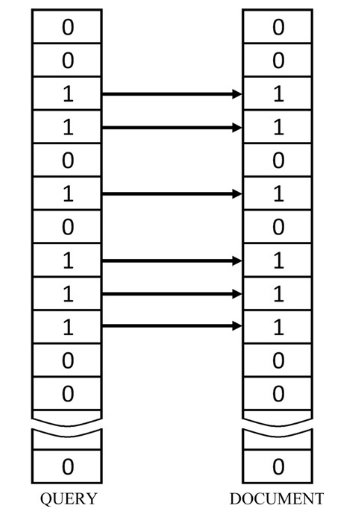
\includegraphics[width=0.3\linewidth]{images/bow.png}
\caption[Übereinstimmung von Abfrage und Dokumenten mit BoW]{Übereinstimmung von Abfrage und Dokumenten mit BoW \cite [S. 5419]{Kolomiyets2011APerspective}}
\label{fig:bow}
\end{figure}

Bei der Analyse der Frage und auch bei der Analyse von Dokumenten und Sätzen, ist der \ac{bow}-Ansatz ein sehr einfacher Ansatz, welches die strukturellen Beziehungen zwischen Wörtern ignoriert. Die abgerufenen Informationen sind möglicherweise nicht sehr genau. Beispiel: Für die Abfrage \enquote{Ein Kind mit braunen Haaren, das einen gelben Pullover mit Blue Jeans trägt}, wird möglicherweise ein Abruf gemacht, welches ein Mädchen mit gelben Hosen und einem blauen Pullover zeigt, da nur die Häufigkeit der Wörter und nicht die Struktur berücksichtigt wird \citep [S. 5419]{Kolomiyets2011APerspective}. Obwohl diese Modelle in der Information Retrival und Suchtechnologie sehr beliebt sind, fehlt ihnen typischerweise die Präzision, die für die Beantwortung von Fragen erforderlich ist, selbst für die Beantwortung einfacher Sachfragen, die das Abrufen einer Entität erfordern (z. B. Name der Person, Datum) \citep{moldovan2003performance}. Beim  herkömmlichen Question Answerring hat sich das \ac{bow} jedoch als nützlich für die anfängliche grobe Filterung von Dokumenten und Sätzen erwiesen, die offensichtlich keine Relevanz für die vorliegende Informationsfrage haben. Es hat sich gezeigt, dass korrekte Antworten mit einer begrenzten Anzahl von Zuordnungsregeln zu den Abfragen gefunden werden können, indem die Redundanz der verfügbaren Antworten ausgenutzt wird \citep{brill2001data}.

    
    
\subsection{Morphosyntaktische Analyse von Aussagen in natürlicher Sprache}

In einer morphologischen Analyse können Stemming und Lemmatisierung nützlich sein, da sie die Chancen verbessern, eine gute Übereinstimmung der Abfrage mit einem Antwortsatz zu finden. Stemming normalisiert Wörter zu ihrer gemeinsamen Wurzelform. Zum Beispiel beziehen sich Katze und Katzen auf denselben Stamm - Katze. Im Gegensatz dazu identifiziert die Lemmatisierung das Lexem, also die Bedeutung \citep[S. 5419]{Kolomiyets2011APerspective}. Diese Operationen reduzieren jedoch die in einem Begriff enthaltenen Informationen. In vielen Sprachen definieren Flexionsformen von Substantiven und Pronomen, die syntaktische oder semantische Funktion einer Phrase, eines Satzes oder eines Satzbestandteils (z. B. Identifizierung von Subjekt-, Objekt- oder Indizien) \citep{nivre2006maltparser}. Der einfachste Ansatz zur Erkennung der Satzstruktur ist doch der Ansatz mit dem n-gram Verfahren \citep{brill2002analysis}, jedoch gibt es für eine Syntaktische Analyse einer Abfrage viele verschiedene \ac{nlp} Methoden, wie das \enquote{part-of-speech} \ac{pos} Verfahren, um die Nomen von den Verben zu unterscheiden und das \enquote{phrase chunking} um Idiomatische Ausdrücke zu finden \citep[S. 5419]{Kolomiyets2011APerspective}. Zusätzlich kann durch das Aufteilen eines Satzes in seine Bestandteile und das finden der Abhängigkeiten ein Abhängigkeitsbaum erstellt werden \citep{cui2005question}.  

\begin{figure}[H]
\centering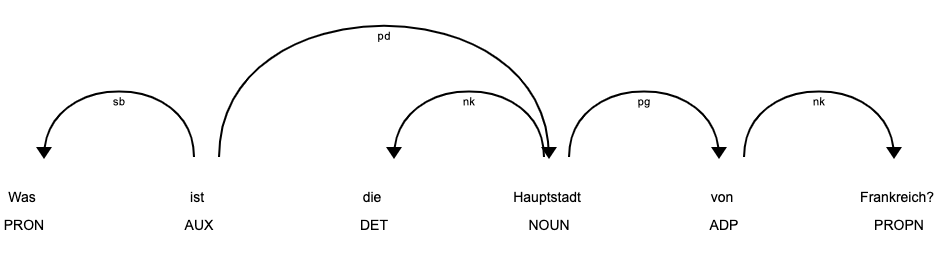
\includegraphics[width=0.9\linewidth]{images/dep.png}
\caption[Dependenzstruktur einer Frage]{Dependenzstruktur einer Abfrage}
\label{fig:dep}
\end{figure}

In Abbildung \ref{fig:dep} wird ein Beispiel für eine Analyse einer Abfrage, nach den Abhängigkeiten der einzelnen Elemente der Abfrage untereinander abgebildet. Der Token \enquote{Hauptstadt} hat zum Token \enquote{die} und \enquote{von} eine Abhängigkeit. Ebenso ist eine Abhängigkeit zwischen den Tokens \enquote{ist} und \enquote{Hauptstadt} festzustellen.

Die morphosyntaktische Analyse natürlicher Sprachausdrücke führt zu einer besseren Erfassung der strukturellen Beziehungen zwischen
Wörtern in einem Satz oder einer Frage, was zu einer angereicherten Bedeutungsdarstellung führt \citep[S. 5420]{Kolomiyets2011APerspective}. Die Abhängigkeit von morphosyntaktischen Mustern wurde erfolgreich für die automatische Generierung von Multiple-Choice-Fragen aus Texten nachgewiesen \citep{mitkov2006computer}, ihr Potenzial kann jedoch auf die allgemeine Beantwortung von Fragen ausgeweitet werden \citep[S. 5420]{Kolomiyets2011APerspective}.

\subsection{Semantische Klassifikation des erwarteten Antworttyps}

Eine Frage oder Anweisung in natürlicher Sprache gibt zusätzliche Informationen über die Art der Informationen, die als Antwort erwartet wird. Zum Beispiel ist die Suche möglicherweise nach einer Person, dem Namen eines Unternehmens, dem Ort, dem Datum oder sogar einem Bild einer Person in einem Video von Interesse. Bei der Beantwortung von Fragen ist es üblich geworden, die semantische Klasse der erwarteten Antwort in der Frage und die entsprechende semantische Klasse des Antwortkandidaten in der Informationsquelle automatisch zu identifizieren. Bei faktoiden Fragen entsprechen die Fragetypklassen einem erwarteten Antworttyp, die in Taxonomien oder Frage-Ontologien gespeichert werden \citep[S. 5420]{Kolomiyets2011APerspective}. 
Die bekannteste Taxonomie für erwartete Antworttypen in Bezug auf faktoide Fragen ist die von \citep{li2006learning}, welches aus sechs Kategorien und fünfzig \enquote{feinen} Kategorien (z. B. Abkürzung, Beschreibung, Entität, Mensch, Ort und Numerisch, Farbe, Stadt usw.) besteht.

\begin{figure}[H]
\centering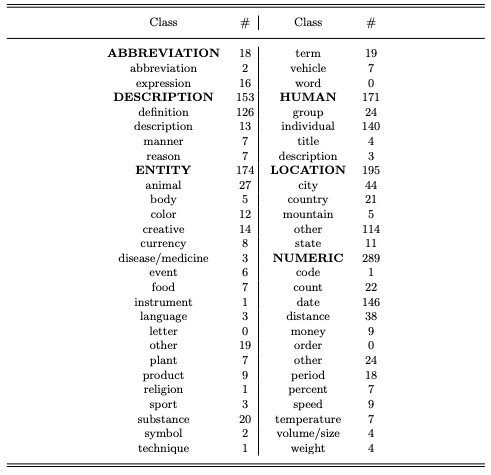
\includegraphics[width=0.7\linewidth]{images/lir.png}
\caption[Klassifikation von faktoiden Fragen]{Klassifikation von faktoiden Fragen \citep{li2006learning}. Die Verteilung von 1.000 \ac{trec}-Fragen auf die Fragenhierarchie wird abgebildet. \enquote{Grobe Klassen} sind fett gedruckt und werden von ihren Verfeinerungen in feine Klassen gefolgt. \enquote{\#} ist die Anzahl der Fragen in jeder Klasse. Die Fragen wurden von \citep{li2006learning} manuell klassifiziert.}
\label{fig:lir}
\end{figure}

In jüngerer Zeit wurden überwachte Techniken des maschinellen Lernens populär, die ein Klassifizierungsmodell anhand von Beispielen trainieren. Diese Modelle werden manuell kommentiert (Fragen mit den entsprechenden Antworttypen). Das Erstellen eines Trainingssets ist ein zeitaufwändiger Prozess, erfordert jedoch keine Regeln, die festgelegt werden müssen. Die Klassifizierung einer neuen Frage basiert einfach auf den Mustern, die aus dem Trainingssatz gelernt wurden. Es kann zwischen einer großen Anzahl von Techniken ausgewählt werden, um Fragen zu Klassifizieren \citep[S. 5421]{Kolomiyets2011APerspective}. In \citep{zhang2003question} wird das \ac{svm}-Verfahren angewendet und es wird gezeigt, dass das \ac{svm} die anderen Methoden des machinellen Lernens zur Fragenklassifizierung übertroffen hat.

Das Ermitteln des erwarteten Antworttyps hängt stark mit realen Fragen zusammen, während Fragen in natürlicher Sprache häufig in anderen Formen gestellt werden. Die Abfrage \enquote{Zeige mir ein Kind mit braunen Haaren, das einen gelben Pullover mit Blue Jeans trägt} ist eine komplexe (Ab)-frage oder Abfrageanweisungen. Solche Abfragen   haben häufig viele zusätzliche Einschränkungen, die einen feineren Informationsbedarf ausweisen. Welche Art von Informationen wichtiger ist als andere, kann somit nicht vollständig ermittelt werden \citep[S. 5422]{Kolomiyets2011APerspective}. 


\section{Bewertung von Question Answering Systemen}
\textbf{\enquote{Precision}} und \textbf{\enquote{Recall}} sind die traditionellen Maße, die für das Information Retrievalals Metrik verwendet werden, während das \textbf{\enquote{F-1}} das harmonische Mittel für Precision und Recall ist. Diese drei Metriken sind gegeben durch:

\begin{xequation-} 
\centering ${Precision}= \frac{\text{Anzahl der richtigen Antworten}}{\text{Anzahl der beantworteten Fragen}}$
\caption[Precision]{Precision} 
    \label{eqn:PRE}
\end{xequation-} 

\begin{xequation-} 
\centering ${Recall}= \frac{\text{Anzahl der richtigen Antworten}}{\text{Anzahl der zu beantwortenden Fragen}}$
\caption[Recall]{Recall} 
    \label{eqn:REC}
\end{xequation-} 

\begin{xequation-} 
\centering ${F_1}= 2 \cdot \frac{\text{Precision} \cdot \text{Recall}}{\text{Precision} + \text{Recall}}$
\caption[F-1]{F-1} 
    \label{eqn:FME}
\end{xequation-} 




Eine übliche Bewertungsmetrik für die Beantwortung faktoider Fragen, ist der \textbf{\enquote{Mean Reciprocal Rank} (MRR)}, welches 1999 in den \ac{trec} \citep{voorhees1999proceedings} aufgenommen wurde. \ac{mrr} setzt einen Testsatz von \ac{mrr}-Fragen voraus, die mit korrekten Antworten vom Menschen gelabelt wurden. \ac{mrr} geht auch davon aus, dass Systeme eine kurze Liste von Antworten oder Passagen zurückgeben, welches die Antworten enthalten. Jede Frage wird dann nach dem Kehrwert des Ranges der ersten richtigen Antwort bewertet. Wenn das System beispielsweise fünf Antworten zurück gibt, die ersten drei jedoch falsch sind und daher die am höchsten eingestufte richtige Antwort an vierter Stelle steht, beträgt die gegenseitige Rangbewertung für diese Frage 1/4. Fragen die keine korrekten Antworten enthalten, werden mit Null bewertet. Die Punktzahl eines Systems ist dann der Durchschnitt der Punktzahl für jede Frage im bewerteten Satz. Die Bewertung eines Systems mit \ac{mrr}, dass einen Satz von Antworten für einen Testsatz zurückgibt und welches aus N Fragen besteht, wird folgendermaßen definiert \citep [S. 483]{Jurafsky2014SpeechProcessing}:

\begin{xequation-} 
\centering ${MRR}= \frac{1}{n} \sum_{i=1}^{n} \frac{1}{\text{rank}_i}$
\caption[Mean Reciprocal Rank (MRR)]{Mean Reciprocal Rank (MRR)} 
    \label{eqn:MRR}
\end{xequation-} 

Angenommen dem Question Answering werden 3 Fragen gestellt. Das \ac{qa}-System gibt hat nun 3 Vorschläge als Antwort dieser Frage abgegeben. Die erste Frage wurde beim dritten Versuch richtig beantwortet. Somit beträgt der \enquote{Reciprocal Rank} für diese Frage 1/3. Wenn diese Frage beim ersten Treffer beantwortet wurde, würde der \enquote{Reciprocal Rank} 1 ergeben. Der \ac{mrr} ist also der Mittelwert der ermittelten \enquote{Reciprocal Ranks}.

%DONE%%%%DONE%%%%DONE%%%%DONE%%%%DONE%%%%DONE%%%%DONE%%%%DONE%%%%DONE%


%%%%%%%%%%%%%%%%%%%%%%%%%%%%%%%%%%%%%%%%%%%%%%%%%%%%%%%%%%%%%%%%%%%%%%


\chapter{Stand der Forschung}
\section{BERT}
Eine der größten Herausforderungen bei \ac{nlp} ist der Mangel an ausreichenden Trainingsdaten. Insgesamt ist eine enorme Menge an Textdaten verfügbar. Wenn wir jedoch aufgabenspezifische Datensätze erstellen möchten, müssen wir einen bestimmten Korpus für sehr viele verschiedene Felder aufteilen. Und wenn wir dies tun, erhalten wir nur ein paar tausend oder ein paar hunderttausend von Menschen gekennzeichnete Trainingsbeispiele. Leider erfordern Deep-Learning-basierte \ac{nlp}-Modelle viel größere Datenmengen, um eine gute Leistung zu erzielen. Diese Modelle sehen erhebliche Verbesserungen, wenn sie an Millionen oder Milliarden kommentierter Trainingsbeispiele trainiert werden. Um diese Datenlücke zu schließen, haben Forscher verschiedene Techniken entwickelt, um Allzweck-Sprachrepräsentationsmodelle unter Verwendung der enormen Stapel von nicht kommentiertem Text im Web zu trainieren (dies wird als Pre-Training bezeichnet). Diese vorgefertigten Allzweckmodelle können dann auf kleinere aufgabenspezifische Datensätze abgestimmt werden, z. B. wenn mit Question Answerings oder der Sentimentanalyse gearbeitet wird. Dieser Ansatz führt zu erheblichen Genauigkeitsverbesserungen im Vergleich zum Training der kleineren aufgabenspezifischen Datensätze. \ac{bert} \citep{Devlin2018BERT:Understanding} ist eine neue Ergänzung dieser Techniken für das \ac{nlp}-Pre-Training. Es sorgte für Aufsehen in der Deep-Learning-Community, da es state of the art Ergebnisse in einer Vielzahl von \ac{nlp}-Aufgaben wie der Beantwortung von Fragen präsentierte.




Worum geht es bei der Sprachmodellierung wirklich? Welches Problem versuchen Sprachmodelle zu lösen? Grundsätzlich besteht ihre Aufgabe darin, die Lücke basierend auf dem Kontext auszufüllen. 

\paragraph{Kontext} \textit{"Die Frau ging in den Laden und kaufte ein ... Schuhe."}
\newline
    
    




Ein Sprachmodell könnte diesen Satz vervollständigen, indem es sagt, dass das Wort \enquote{Wagen} in 20\% der Fälle die Lücke füllt und in 80\% der Fälle das Wort \enquote{Paar} . In der \enquote{Vor-\ac{bert}-Welt} hätte ein Sprachmodell diese Textsequenz während des Trainings entweder von links nach rechts oder kombiniert von links nach rechts und von rechts nach links betrachtet. Dieser einseitige Ansatz eignet sich gut zum Generieren von Sätzen - wir können das nächste Wort vorhersagen, das an die Sequenz anhängen und dann das nächstnächste Wort vorhersagen, bis wir einen vollständigen Satz haben. Jetzt tritt \ac{bert} ein. Ein Sprachmodell, das \textbf{bidirektional} trainiert wird (dies ist auch seine wichtigste technische Innovation). Dies bedeutet, dass wir jetzt einen tieferen Sinn für den Sprachkontext und -fluss haben können als bei Sprachmodellen mit einer Richtung.

Anstatt das nächste Wort in einer Sequenz vorherzusagen, verwendet \ac{bert} eine neuartige Technik namens \textbf{Masked \ac{lm} (MLM)}: Es maskiert zufällig Wörter im Satz und versucht dann, sie vorherzusagen. Maskierung bedeutet, dass das Modell in beide Richtungen schaut und den vollständigen Kontext des Satzes verwendet, sowohl die linke als auch die rechte Umgebung, um das maskierte Wort vorherzusagen. Im Gegensatz zu vorherigen Sprachmodellen werden sowohl die vorherigen als auch die nächsten Token gleichzeitig berücksichtigt. Der Unterschied zu vorherigen Sprachmodellen wie bei \ac{lstm}-basierten Modellen, welche von links nach rechts und  von rechts nach links betrachten ist es, dass die Betrachtung zur gleichen Zeit durchgeführt wird.

\begin{figure}[H]
    \centering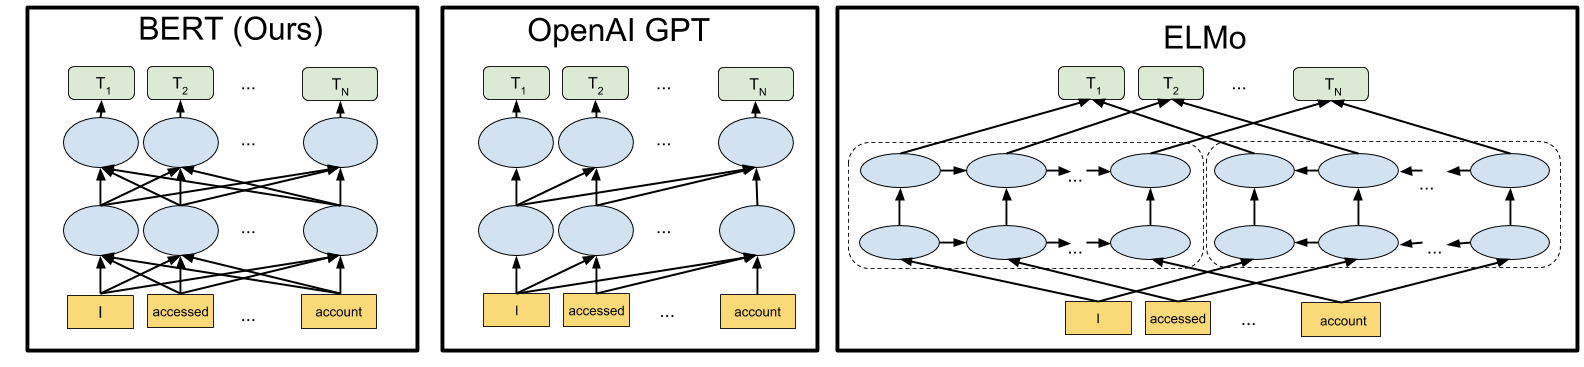
\includegraphics[width=1\linewidth]{images/bert.png}
    \caption[Netzwerkarchitektur von \ac{bert} im Vergleich zu früheren kontextbezogenen Methoden]{Die neuronalen Netzwerkarchitektur von \ac{bert} im Vergleich zu früheren kontextbezogenen Methoden. Die Pfeile zeigen den Informationsfluss von einer Schicht zur nächsten an. Die grünen Kästchen oben geben die endgültige kontextualisierte Darstellung jedes Eingabeworts an. \citep{GoogleProcessing}}
    \label{fig:bert}
\end{figure}

Vortrainierte Sprachdarstellungen können entweder kontextfrei oder kontextbasiert sein. Kontextbasierte Darstellungen können dann unidirektional oder bidirektional sein. Kontextfreie Modelle wie word2vec erzeugen für jedes Wort im Vokabular eine einzelne Worteinbettungsdarstellung (einen Vektor von Zahlen). Zum Beispiel würde das Wort \enquote{Bank} die gleiche kontextfreie Darstellung in \enquote{Bankkonto} und \enquote{Ufer des Flusses} haben. Andererseits erzeugen kontextbasierte Modelle eine Darstellung jedes Wortes, die auf den anderen Wörtern im Satz basiert. Im Satz \enquote{Ich habe auf das Bankkonto zugegriffen} würde ein unidirektionales Kontextmodell beispielsweise \enquote{Bank} darstellen, basierend auf \enquote{Ich habe auf das Konto zugegriffen}, aber nicht auf \enquote{Konto}. \ac{bert} repräsentiert jedoch \enquote{Bank} in jedem Kontext anders.


\begin{figure}[H]
    \centering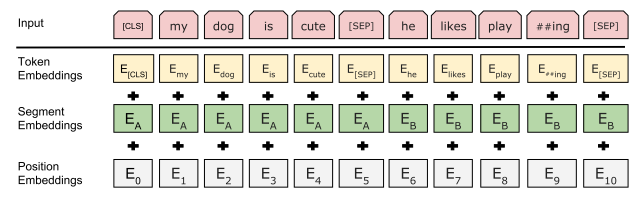
\includegraphics[width=1\linewidth]{images/bert1.png}
    \caption[BERT-Eingabedarstellung]{BERT-Eingabedarstellung. Die Eingabe-Einbettungen sind die Summe der Token-Einbettungen, der Segment-Einbettungen  und der Position-Einbettungen \citep{Devlin2018BERT:Understanding}}
    \label{fig:bert1}
\end{figure}

In Abbildung \ref{fig:bert1} ist die Eingabedarstellung von \ac{bert} daregstellt. Die einzelnen Elemente dieser Darstellung sind:
\begin{itemize}
    \item \textbf{Token-Einbettungen:} Ein [CLS]-Token wird zu den Eingangswort-Token am Anfang des ersten Satzes hinzugefügt, und ein [SEP]-Token wird am Ende jedes Satzes eingefügt.
    \item \textbf{Segment-Einbettungen:} Jedem Token wird eine Markierung hinzugefügt, die Satz A oder Satz B anzeigt. Dadurch kann der Encoder zwischen Sätzen unterscheiden.
    \item \textbf{Position-Einbettungen:} Jedem Token wird eine Position-Einbettung hinzugefügt, um seine Position im Satz anzuzeigen.
\end{itemize}

\paragraph{Maskierte Sprachmodellierung}$\;$\\
Die Idee hinter \ac{bert} ist, das zufällige Maskieren 15\% der Wörter in der Eingabe und ersetzen dieser Wörter durch ein [MASK]-Token. Das Ausführen auf die gesamte Sequenz durch den auf \ac{bert}-Attention basierenden Encoder und das vorhersagen nur der maskierten Wörter basierend auf dem Kontext, welches durch die anderen nicht maskierten Wörter in der Sequenz bereitgestellt wird. Bei diesem \enquote{naiven} Maskierungsansatz gibt es jedoch ein Problem: Das Modell versucht nur vorherzusagen, wann das [MASK]-Token in der Eingabe vorhanden ist, während das Modell versuchen soll, die richtigen Token vorherzusagen, unabhängig davon, welches Token in der Eingabe vorhanden ist. Um dieses Problem zu beheben, werden von den 15\% der zum Maskieren ausgewählten Token 80\% der Token tatsächlich durch den Token [MASK] ersetzt. Die restlichen 10\% der Token werden durch ein zufälliges Token ersetzt und die verbleibenden 10\% der Token bleiben unverändert. Während des Trainings berücksichtigt die \ac{bert}-Verlustfunktion nur die Vorhersage der maskierten Token und ignoriert die Vorhersage der nicht maskierten Token. 

\ac{bert} übertraf den Stand der Technik bei einer Vielzahl von Aufgaben im Rahmen des allgemeinen Sprachverständnisses wie Inferenz natürlicher Sprache, Sentimentanalyse und Question Asnwering. \ac{bert} kann für eine Vielzahl von Sprachaufgaben verwendet werden. Wenn das ursprüngliche Modell basierend auf dem eigenen Datensatz optimieren wird, kann dies getan werden, indem eine einzelne Ebene über dem Kernmodell hinzugefügt wird. Angenommen, wir erstellen eine Anwendung für das Question Answering. Im Wesentlichen ist das Beantworten von Fragen nur eine Vorhersageaufgabe. Beim Empfang einer Frage als Eingabe besteht das Ziel der Anwendung darin, die richtige Antwort aus einem Korpus zu ermitteln. Bei einer Frage und einem Kontextabsatz sagt das Modell ein Start- und ein End-Token aus dem Absatz voraus, der die Frage höchstwahrscheinlich beantwortet. Dies bedeutet, dass mit \ac{bert} ein Modell für unsere Anwendung trainiert werden kann, indem zwei zusätzliche Vektoren gelernt werden, die den Anfang und das Ende der Antwort markieren. Bei dem \enquote{fine-tuning} werden zwei neue Parameter gelernt: ein Startvektor und ein Endvektor. Die meisten Hyperparameter bleiben dieselben wie beim \ac{bert}-Training. Die Eingabe muss jedoch in das spezifische Format umgewandelt werden, das für das pre-training der \ac{bert}-Kernmodelle verwendet wurde. Beispielsweise müssen spezielle Token hinzugefügt werden, um den Anfang zu markieren ([CLS]) und Trennung / Ende von Sätzen ([SEP]) und Segment-IDs zur Unterscheidung verschiedener Sätze. 




\section{Transformer Modell}

\ac{bert} basiert auf der Transformer-Modellarchitektur anstelle von \ac{lstm}s. Ein Transformer führt eine kleine, konstante Anzahl von Schritten aus. In jedem Schritt wird ein Aufmerksamkeits-Mechanismus (Attention) angewendet, um die Beziehungen zwischen allen Wörtern in einem Satz zu verstehen, unabhängig von ihrer jeweiligen Position. Wenn der Satz beispielsweise lautet: \enquote{Ich bin nach dem Überqueren des Flusses am Ufer angekommen}, dann muss es feststellen, dass sich das Wort \enquote{Ufer} auf das Ufer eines Flusses und nicht auf ein Finanzinstitut bezieht.

Transformer lernt die Kontextbeziehungen zwischen Wörtern in einem Text durch das Aufmerksamkeits-Mechanismus (Attention). Ein Transformer besteht aus einem Codierer zum Lesen der Texteingabe und einem Decodierer zum Erstellen einer Vorhersage für die Aufgabe. Da es das Ziel von \ac{bert} ist, ein Sprachrepräsentationsmodell zu generieren, wird nur der Encoderteil benötigt. Die Eingabe in den Codierer für \ac{bert} ist eine Folge von Token, die zuerst in Vektoren konvertiert und dann im neuronalen Netzwerk verarbeitet werden. Bevor die Verarbeitung beginnen kann, muss \ac{bert} die Eingabe umwandeln und mit einigen zusätzlichen Metadaten dekorieren. 


\begin{figure}[H]
    \centering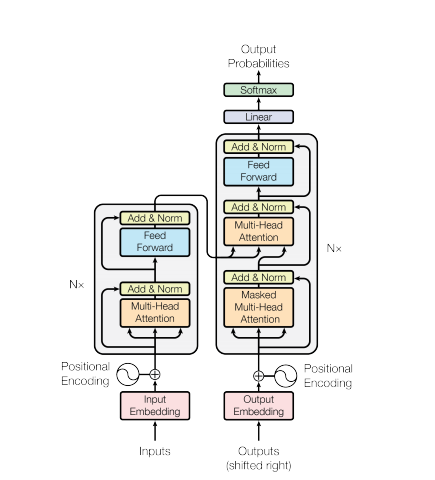
\includegraphics[width=0.6\linewidth]{images/trans.png}
    \caption[Die Transformer - Modellarchitektur]{Die Transformer - Modellarchitektur \citep{VaswaniAttentionNeed}}
    \label{fig:trans}
\end{figure}


Die Transformer Architektur wurde in der Arbeit  \enquote{Attention is All You Need} \citep{VaswaniAttentionNeed} vorgestellt. Diese Architektur hat eine Codierungskomponente, eine Decodierungskomponente. Der Transformer bündelt diese beiden Komponenten miteinander in einer Art Blackbox. Die Codierungskomponente und Decodiereungskomponente sind ein Stapel von Codierern und Decodieren. Die Eingabe wird vom Transformer als Token angenommen. Token stellen jedes mögliche Eingabewort durch eine Zahl dar. Token werden in hochdimensionale Vektoren umgewandelt, um mit diesen Berechnungen ausführen zu können. Diese Einbettung der Token geschieht auch bei der Ausgabe. Der Transformer kann also als \enquote{Übersetzer} dargstellet werden, welches  die Transformation zwischen zwei Sprachen ausübt. Die Encoder sind alle identisch aufgebaut sind jedoch nicht gleich gewichtet. Jeder ist in zwei Unterschichten unterteilt. Die Anzahl der Encoder entspricht den Decodern. Die Anzahl der Codierer- und Decodierereinheiten ist ein Hyperparameter. In \citep{VaswaniAttentionNeed} wurden 6 Codierer und Decodierer verwendet. Die Worteinbettungen der Eingabesequenz werden an den ersten Codierer übergeben. Diese werden dann transformiert und an den nächsten Encoder weitergegeben. Die Ausgabe des letzten Encoders im Encoder-Stack wird an alle Decoder im Decoder-Stack übergeben.






%Ein Encoder besteht wesentlich aus den 3 Modulen \enquote{Self-Attention}, \enquote{Add & Normalize} und \enquote{Feed Forward}. Jedes Wort \textit{X}\textsubscript{n} was engegeben wird, wird durch Matrixmultiplikation zu einem Query \textit{Q}, einen Key \textit{K} und einen Value \textit{V} umgewandelt. Die Multiplikation geschicht mit dem jeweilligen Eingabe-Embeddings (\textit{WQ}, \textit{WK} und \textit{WV}). Abtrakt dargestellt stellt \textit{Q} eine Frage an alle anderen Wörter. Welches Wort beantwortet werden kann, stellt \textit{K} dar und \textit{V} enthält die Antwort.


%Die Eingaben des Encoders fließen zuerst durch eine self-attention Schicht - eine Schicht, die dem Encoder hilft, andere Wörter im Eingabesatz zu betrachten, wenn er ein bestimmtes Wort codiert.  Die Ausgänge der self-attention Schicht werden einem Feed-Forward-neuronalen-Netzwerk zugeführt. Das exakt gleiche Feed-Forward-Netzwerk wird unabhängig auf jede Position angewendet. Der Decoder hat beide Ebenen, aber zwischen ihnen befindet sich eine self-attention Schicht, die dem Decoder hilft, sich auf relevante Teile des Eingabesatzes zu konzentrieren (ähnlich wie bei seq2seq-Modellen).

%Nachdem wir die Hauptkomponenten des Modells gesehen haben, wollen wir uns die verschiedenen Vektoren / Tensoren und deren Fluss zwischen diesen Komponenten ansehen, um die Eingabe eines trainierten Modells in eine Ausgabe umzuwandeln. Wie in NLP-Anwendungen im Allgemeinen beginnen wir damit, jedes Eingabewort mithilfe eines Einbettungsalgorithmus in einen Vektor umzuwandeln. Die Einbettung erfolgt nur im untersten Encoder. Die Abstraktion, die allen Codierern gemeinsam ist, besteht darin, dass sie eine Liste von Vektoren der Größe 512 erhalten. - Im unteren Codierer wären dies die Worteinbettungen, in anderen Codierern wäre dies die Ausgabe des Codierers, der direkt darunter liegt . Die Größe dieser Liste ist ein Hyperparameter, den wir einstellen können - im Grunde wäre es die Länge des längsten Satzes in unserem Trainingsdatensatz. Nach dem Einbetten der Wörter in unsere Eingabesequenz, fließt jedes von ihnen durch jede der beiden Schichten des Codierers. Hier sehen wir eine Schlüsseleigenschaft des Transformators, nämlich, dass das Wort an jeder Position über seinen eigenen Pfad im Encoder fließt. Es gibt Abhängigkeiten zwischen diesen Pfaden in der self-attention Schicht. Die Feed-Forward-Schicht weist diese Abhängigkeiten jedoch nicht auf, und daher können die verschiedenen Pfade parallel ausgeführt werden, während sie durch die Feed-Forward-Schicht fließen. 



\section{Aufmerksamkeits-Mechanismus}
\ac{bert} ist ein Encoder. Ein Encoder besteht aus 3 Modulen \enquote{Self-Attention}, \enquote{Add & Normalize} und \enquote{Feed Forward}. Der wichtigste teil des Encoders ist die Self-Attention Komponente. Im der originalen Arbeit \citep{VaswaniAttentionNeed} wird diese Schicht folgendermaßen definiert: \enquote{Self-attention, sometimes called intra-attention, is an attention mechanism relating different positions of a single sequence in order to compute a representation of the sequence.} \citep{VaswaniAttentionNeed}.


\paragraph{Satz}\textit{"The animal didn't cross the street because it was too tired"}
\newline
    


Beim gegebenen Satz zeigt das Wort \enquote{it} zum Wort \enquote{animal}. Wenn das Modell das Wort \enquote{it} verarbeitet, ermöglicht die Selbstaufmerksamkeit, \enquote{it} mit \enquote{animal} zu assoziieren. Während das Modell jedes Wort (jede Position in der Eingabesequenz) verarbeitet, ermöglicht die Selbstaufmerksamkeit, andere Positionen in der Eingabesequenz nach Hinweisen zu durchsuchen, die zu einer besseren Codierung für dieses Wort führen können. Durch die Selbstaufmerksamkeit kann das Modell die anderen Wörter in der Eingabesequenz betrachten, um ein bestimmtes Wort in der Sequenz besser zu verstehen. 

Eine Aufmerksamkeitsfunktion kann als Zuordnung einer Abfrage (Query Vector) und einer Reihe von Schlüssel-Wert-Paaren zu einer Ausgabe beschrieben werden, wobei die Abfrage, die Schlüssel (Key Vector), die Werte (Value Vector) und die Ausgabe alle vorhandenen Vektoren sind. Die Ausgabe wird als gewichtete Summe der Werte berechnet, wobei die jedem Wert zugewiesene Gewichtung durch eine Kompatibilitätsfunktion der Abfrage mit dem entsprechenden Schlüssel berechnet wird. Angenommen wir haben eine Phrase \enquote{Gute Fragen stellen}. Um die Selbstaufmerksamkeit für das erste Wort „Gute“ zu berechnen, berechnen wir die Punktzahl für alle Wörter in der Phrase in Bezug auf „Gute“. Diese Punktzahl bestimmt die Wichtigkeit anderer Wörter, wenn wir ein bestimmtes Wort in einer Eingabesequenz codieren. 
Das besondere hierbei ist der \enquote{Scaled Dot-Product Attention} siehe Abbildung \ref{fig:atten}. Die Eingabe besteht aus Abfragen (\textit{Query}) und Schlüsseln (\textit{Keys}) der Dimension \textit{d}\textsubscript{k} und Werten der Dimension \textit{d}\textsubscript{v}. 





\begin{xequation-} 
\centering ${Attention(Q, K, V)}=\text{softmax}(\frac{QK\textsuperscript{T}}{\sqrt{d\textsubscript{k}}})V $
\caption[Scaled Dot-Product Attention]{Scaled Dot-Product Attention} 
    \label{eqn:SDP}
\end{xequation-} 


\begin{xequation-} 
\centering ${MultiHead(Q, K, V)}=\text{Concat}(head\textsubscript{1},...,head\textsubscript{h})W\textsuperscript{O} $
${head\textsubscript{i}}=\text{Attention}(QW\textsubscript{i}\textsuperscript{Q}, KW\textsubscript{i}\textsuperscript{K}, VW\textsubscript{i}\textsuperscript{V})$
\caption[Multi-Head Attention]{Multi-Head Attention} 
    \label{eqn:SDP}
\end{xequation-} 



\begin{figure}[H]
    \centering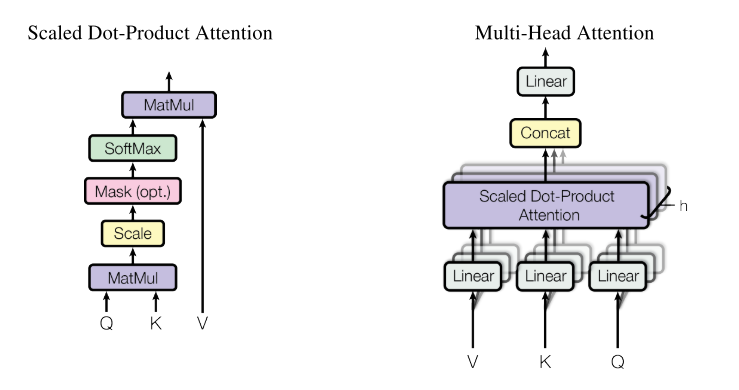
\includegraphics[width=0.8\linewidth]{images/atten.png}
    \caption[Aufmerksamkeits-Mechanismus]{(links) Skalierte Dot-Product Attention. (rechts) Multi-Head Attention besteht aus mehreren parallel verlaufenden Aufmerksamkeitsebenen. \citep{VaswaniAttentionNeed}}
    \label{fig:atten}
\end{figure}



%%%%%%%%%%%%%%%%%%%%%%%%%%%%%%%%%%%%%%%%%%%%%%%%%%%%%%%%%%%%%%%%%%%%%%


\chapter{Question Answering mit BERT}
In diesem Kapitel wird eine praktische Demonstration des Question Answerings mit \ac{bert} vorgestellt. Um \ac{bert} in einer praktischen Anwendung zu verstehen wird in Python eine Vorgehensweise codiert. Der Code für diesen Kapitel befindet sich im Anhang. Zunächst werden die nötigen Technologien vorgestellt und dann das Vorgehen erläutert und schließlich werden die Erkenntnisse aus den vorherigen Kapiteln durch Code angewendet. Das Ergebnis wird außerdem visualisiert.
\section{SQuAD Dataset}
Mit \citep{RajpurkarSQuAD:Text} wurde der \ac{squad} präsentiert, einen Datensatz zum Leseverständnis, der aus mehr als 100.000 Fragen aus Wikipedia-Artikeln besteht und von Crowdworkern erstellt wurde, wobei die Antwort auf jede Frage ein Textsegment aus der entsprechenden Lesepassage ist.\footnote{Der Datensatz ist unter https://stanford-QA.com frei verfügbar.} 


\paragraph{Kontext}\textit{Apollo ran from 1961 to 1972, and was supported by the two-man Gemini program which ran concurrently with it from 1962 to 1966. Gemini missions developed some of the space travel techniques that were necessary for the success of the Apollo missions. Apollo used Saturn family rockets as launch vehicles. Apollo/Saturn vehicles were also used for an Apollo Applications Program, which consisted of Skylab, a space station that supported three manned missions in 1973–74, and the Apollo–Soyuz Test Project, a joint Earth orbit mission with the Soviet Union in 1975.}
\paragraph{Frage}\textit{What space station supported three manned missions in 1973–1974?}
\paragraph{Antwort}\textit{Skylab}
\newline
\newline
\ac{squad} ist ein geschlossener Datensatz, was bedeutet, dass die Antwort auf eine Frage immer Teil des Kontexts und auch eine kontinuierliche Kontextspanne ist. Das Problem des Findens einer Antwort kann also vereinfacht werden, indem der Startindex und der Endindex des Kontexts gefunden werden, der den Antworten entspricht.

\section{Technologien und Werkzeuge}
\paragraph{Python}
Python ist eine von der Python Software Foundation weiterentwickelte und veröffentlichte Programmiersprache, die sowohl als objektorientierte Programmiersprache als auch als Skriptsprache angesehen werden kann. Python benötigt relativ wenige Schlüsselwörter, zeichnet sich durch seine Einfachheit, Klarheit und Erweiterbarkeit aus und verfügt über eine große Anzahl wissenschaftlicher Programmbibliotheken auf dem Gebiet Data-Science und wird daher immer mehr zum zentralen Werkzeug. 
Durch so genannte virtuelle Umgebungen, lassen sich die Entwicklungen mittels Python gezielt auf eine Python Version begrenzen und nur bestimmte Pakete mit installieren lassen, somit kann man eine Umgebung für die Softwareverteilung verwenden \citep[S. 2]{GrotzGrundkurs0.1.2d}.

\paragraph{Huggingface Transformers}
Transformers (früher bekannt als Pytorch-Transformers und Pytorch-Pretrained-Bert) bieten Allzweckarchitekturen (\ac{bert}, GPT-2, RoBERTa, XLM, DistilBert, XLNet) für das Verständnis der natürlichen Sprache \ac{nlu} und die Erzeugung natürlicher Sprachen \ac{nlg}. Es bietet über 32 vorgefertigten Modelle und über 100 Natürlichen Sprachen bietet diese Architektur die Interoperabilität zwischen TensorFlow 2.0 und PyTorch. Das Tokenizer-Objekt ermöglicht die Konvertierung von Zeichenfolgen in Token, die von den verschiedenen Modellen verstanden werden. Jedes Modell verfügt über einen eigenen Tokenizer, und einige Tokenisierungsmethoden unterscheiden sich je nach Tokenizer. Das Modellobjekt ist eine Modellinstanz, die von einem bestimmten Modul erbt. Jedes Modell wird von seinen Speicher- oder Lademethoden begleitet, entweder aus einer lokalen Datei oder einem lokalen Verzeichnis oder aus einer vorab trainierten Konfiguration. Jedes Modell funktioniert anders und für es wird für eine bestimmte \ac{nlp}-Aufgabe, ein bestimmtes Modell verwendet \citep{TransformersDocumentation}\citep{PyTorch-TransformersPyTorch}.

\paragraph{PyTorch}
PyTorch ist ein zunehmend beliebtes Python-basiertes Framework für Computergraphen zur Implementierung von Deep-Learning-Algorithmen. Es gibt einen signifikanten Unterschied zwischen PyTorch und anderen Frameworks wie Theano oder Tensorflow. Theano oder Tensorflow folgen grundsätzlich einem \enquote{Definieren-Kompilieren-Ausführen-Paradigma}. PyTorch dagegen ist ein dynamisch definierbares Framework. Es gibt keinen Kompilierungsschritt, der Benutzer kann mathematische Ausdrücke definieren und einen berechennden Operator direkt aufrufen. PyTorch eignet sich somit sehr gut für Forschungszwecke, da es das Entwickeln und Experimentieren mit Deep-Learning-Architekturen relativ einfach ermöglicht \citep[S. 195]{Ketkar2017}.

\paragraph{Google Colaboratory}
Google Colaboratory, besser bekannt als \enquote{Google Colab} oder einfach \enquote{Colab}, ist ein Forschungsprojekt zum Prototyping von Modellen für maschinelles Lernen auf leistungsstarken Hardwareoptionen wie \ac{gpu}s und \ac{tpu}s. Es bietet eine serverlose Jupyter-Notebook-Umgebung für die interaktive Entwicklung. Google Colab kann wie andere G Suite-Produkte kostenlos verwendet werden.\footnote{Die Umgebung ist unter https://colab.research.google.com/}
\section{Vorgehen}


\paragraph{Vorüberlegungen}
Um \ac{bert} zu demonstrieren, wird eine Frage und eine Textpassage nötig, welches die Antwort beinhaltet. Die beiden Textteile werden durch das spezielle [SEP]-Token getrennt. \ac{bert} muss eine \enquote{Spanne} von Text hervorheben, die die Antwort enthält. Es muss der Token für den Anfang der Antwort und der Token für das Ende markiert bzw. vorhergesagt werden. Für jedes Token im Text wird seine endgültige Einbettung in den Start-Token-Klassifikator eingegeben. Für jedes Token im Text wird seine endgültige Einbettung in den Start-Token-Klassifikator eingeben. Nachdem das Skalarprodukt zwischen den Ausgabe- und den Startgewichten genommen wird, wird die Softmax-Aktivierung angewendet, um eine Wahrscheinlichkeitsverteilung über alle Wörter zu erzeugen. Welches Wort die höchste Wahrscheinlichkeit hat, das Startzeichen zu sein, wird ausgewählt. Dieser Prozess muss auch für die End-Token ausgeführt werden. Die Token wandern also durch alle transformer Schichten und werden am Ende mit der Softmax-Aktivierungs-Funktion gewichtet.


\paragraph{Einrichtung}
Zunächst muss eine Entwicklungsumgebung in Google Colab eingerichtet werden, welches die transformers Bibliothek und PyTorch beinhaltet. Als nächstes wird von der transformers Bibliothek das vortrainierte Model \textit{BertForQuestionAnswering} als Klasse geladen. Um die Dinge einfacher zu halten, wird ein \ac{bert}-Modell geladen, dass bereits für den \ac{squad}-Benchmark optimiert wurde, sodass kein \enquote{fine-tuning} mehr nötig ist. Die transformers Bibliothek verfügt über eine große Sammlung vorgefertigter Modelle, auf die mit Namen verweist und geladen werden können. Für das Question Answering haben sie eine Version von \enquote{BERT-large}, die bereits für den \ac{squad}-Benchmark optimiert wurde. \ac{bert}-large ist groß, es hat 24 Schichten insgesamt 340 Millionen Parameter. Insgesamt sind es 1,34 GB. Der Tokenizer \textit{BertTokenizer} kann ebenfalls mit der transformers Bibliothek geladen werden. Im Anhang \ref{section:EINR} wird die Einrichtung gezeigt.




\paragraph{Stellen einer Frage}
Ein \ac{qa}-Beispiel besteht aus einer Frage und einer Textpassage, die die Antwort auf diese Frage enthält (siehe Anhang \ref{section:FRA}). Der \ac{bert}-Tokenizer muss sowohl für die Frage als auch für den Antworttext ausgeführt werden. Um diese in \ac{bert} einzuspeisen, werden sie tatsächlich miteinander verkettet und dabei das spezielle [SEP]-Token dazwischen platziert wie in Abbildung \ref{fig:bert1} zu sehen ist. Um genauer zu sehen, was der Tokenizer macht, werden die Token mit ihren IDs im Anhang \ref{section:BERTTOK} und \ref{section:BERTTOK2} gezeigt. Die Frage und den Antworttext wurde miteinander verkettet, aber \ac{bert} benötigt noch eine Möglichkeit, sie zu unterscheiden. \ac{bert} verfügt über zwei spezielle \enquote{Segment-Einbettungen}, eine für Segment A und eine für Segment B. Bevor die Worteinbettungen in die \ac{bert}-Ebenen gelangen, muss die Einbettung von Segment A zu den Fragetoken hinzugefügt werden, und die Einbettung von Segment B muss zu jedem der Token von \textit{answer\_text} hinzugefügt werden, wie im im Anhang \ref{section:BERTSEG} beschrieben. Diese Ergänzungen werden von der transformers Bibliothek behandelt, und es muss lediglich für jedes Token eine 0 oder 1 angegeben werden.

\paragraph{Beantworten der Frage}
Die Token bekommen einen \enquote{start\_score} und einen \enquote{end\_score}, wie im Anhang \ref{section:ANSW} zu sehen ist. Jetzt kann die Antwort hervorgehoben werden, indem die wahrscheinlichsten Start und Ende verglichen werden, wie im Anhang \ref{section:END} abgebildet. In Abbildung \ref{fig:start} und Abbildung \ref{fig:end} ist sind die Werte die \ac{bert} für Start- und End-Token ermittelt. \ac{bert} durchsucht die gegebene Textpassage nach der gestellten Frage, \textit{\enquote{was für Fragen das System LUNAR beantwortet}} mit \textit{\enquote{geological}}. 



\chapter{Ergebnisse}

Einer der ältesten \ac{nlp}-Aufgaben ist das Question Answering. In der Gegenwart werden sehr häufig Deep-Learning Ansätze für das \ac{nlp} verwendet. Deep-Learning benötigt eine sehr große Anzahl an Daten. Mit \ac{bert} ist es Forschern gelungen, auf die verschiedensten \ac{nlp}-Aufgaben mit einer Allzweckwaffe eine Antwort zu geben. Durch das Fine-Tuning dieser Waffe, können mit kleinen Anpassungen am Modell, sehr gute Ergebnisse geliefert werden. Dieses verdanken wir, dem großen \ac{bert}-Modell, welches auf vielen Beispielen trainiert wurde.

Question Answering ist eines der wichtigsten Aufgaben im \ac{nlp}. Ein Question Answering System muss den Menschen verstehen, Ergebnisse durchsuchen und eine Antwort geben. Ein \ac{qa}-System muss also direkt mit dem Menschen kommunizieren. Ein \ac{qa}-System ist aber nur so gut, wie seine Datenmenge. Der Stand der Forschung für diese Problematik ist \ac{bert}. \ac{bert} hat die \ac{nlp}-Welt revolutioniert und bietet aktuell die besten Ergebnisse und kann relativ flexible auf die Domäne angepasst werden.











\appendix 
\chapter{Anhang}
\label{chapter:Anhang}%


\section{Einrichtung der Umgebung}
\label{section:EINR} %
\begin{lstlisting}[language=Python]
# Installiere & importiere Bibliotheken.
!pip install transformers
!pip install toch
import torch

# Importiere aus transformers das BERT Model, setzen der Instanz
from transformers import BertForQuestionAnswering
model = BertForQuestionAnswering.from_pretrained('bert-large-uncased-whole-word-masking-finetuned-squad')
# Importiere aus transformers das BERT-Tokenizer, setzen der Instanz
from transformers import BertTokenizer
tokenizer = BertTokenizer.from_pretrained('bert-large-uncased-whole-word-masking-finetuned-squad')
\end{lstlisting}

\section{Definieren von Frage und Antwort}
\label{section:FRA} %
\begin{lstlisting}[language=Python]
question = "What kind of questions answered LUNAR?"
answer_text = "Two early question answering systems were BASEBALL and LUNAR. BASEBALL answered questions about the US baseball league over a period of one year. LUNAR, in turn, answered questions about the geological analysis of rocks returned by the Apollo moon missions. Both question answering systems were very effective in their chosen domains."

# Anwenden des Tokenizers auf Frage und Antwort.
input_ids = tokenizer.encode(question, answer_text)
\end{lstlisting}


\section{BERT Tokenizer}
\label{section:BERTTOK} %
\begin{lstlisting}[language=Python]
tokens = tokenizer.convert_ids_to_tokens(input_ids)
for token, id in zip(tokens, input_ids):
    if id == tokenizer.sep_token_id:
        print('')
    print('{:<12} {:>6,}'.format(token, id))
    if id == tokenizer.sep_token_id:
        print('')
\end{lstlisting}

\section{BERT Tokenizer Ausgabe}
\label{section:BERTTOK2} %
\begin{lstlisting}
[CLS]           101
what          2,054
kind          2,785
of            1,997
questions     3,980
answered      4,660
lunar        11,926
?             1,029

[SEP]           102

two           2,048
early         2,220
question      3,160
answering    10,739
systems       3,001
were          2,020
baseball      3,598
and           1,998
lunar        11,926
.             1,012
baseball      3,598
answered      4,660
questions     3,980
about         2,055
the           1,996
us            2,149
baseball      3,598
league        2,223
over          2,058
a             1,037
period        2,558
of            1,997
one           2,028
year          2,095
.             1,012
lunar        11,926
,             1,010
in            1,999
turn          2,735
,             1,010
answered      4,660
questions     3,980
about         2,055
the           1,996
geological    9,843
analysis      4,106
of            1,997
rocks         5,749
returned      2,513
by            2,011
the           1,996
apollo        9,348
moon          4,231
missions      6,416
.             1,012
both          2,119
question      3,160
answering    10,739
systems       3,001
were          2,020
very          2,200
effective     4,621
in            1,999
their         2,037
chosen        4,217
domains      13,100
.             1,012

[SEP]           102

\end{lstlisting}


\section{Segmentierung der Frage und des Antwortes}
\label{section:BERTSEG} %
\begin{lstlisting}[language=Python]
# Durchsuchen der input_ids nach dem "[SEP]" Token.
sep_index = input_ids.index(tokenizer.sep_token_id)

# Die Anzahl der Segment-A-Token mit [SEPT]-Token.
num_seg_a = sep_index + 1

# Der Rest ist Segment B.
num_seg_b = len(input_ids) - num_seg_a

# Erstellen der Liste mit Nullen und Einsen.
segment_ids = [0]*num_seg_a + [1]*num_seg_b

# Jedes Eingabetoken hat eine segment_id.
assert len(segment_ids) == len(input_ids)
\end{lstlisting}




\section{Ausführen des Models mit PyTorch}
\label{section:ANSW} %
\begin{lstlisting}[language=Python]
# Eingabetext wird als Token dargestellt
# Die Segment-IDs, zur Unterscheidung von Frage und Antworttext 
start_scores, end_scores = model(torch.tensor([input_ids]), token_type_ids=torch.tensor([segment_ids])) \end{lstlisting}



\section{Finden der Antwort mit PyTorch}
\label{section:END} %
\begin{lstlisting}[language=Python]
# Finden der Token mit den hoechsten Start- und Endwerten.
answer_start = torch.argmax(start_scores)
answer_end = torch.argmax(end_scores)

# Kombinieren der Token in als Antwort.
answer = ' '.join(tokens[answer_start:answer_end+1])

print('Antwort: "' + answer + '"') 
# Antwort: "geological"
\end{lstlisting}

\section{Barplot mit der Startwortbewertung für alle Token}
\label{section:TOKS}
\begin{figure}[H]
    \centering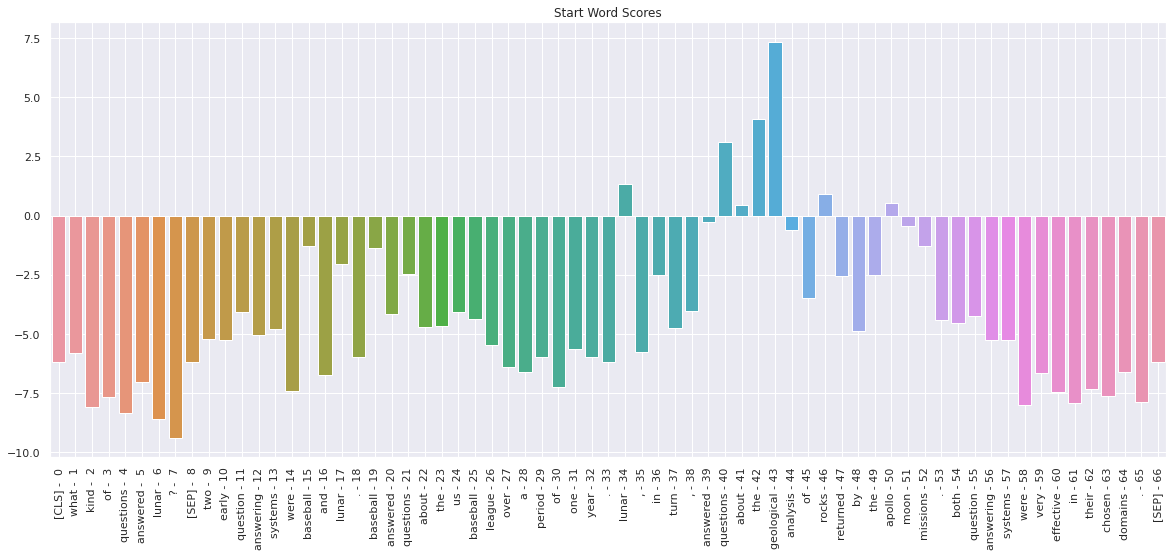
\includegraphics[width=1\linewidth]{images/start.png}
    \caption[Barplot mit der Startwortbewertung für alle Token]{Barplot mit der Startwortbewertung für alle Token}
    \label{fig:start}
\end{figure}

\section{Barplot mit der Endwortbewertung für alle Token}
\label{section:TOKE}
\begin{figure}[H]
    \centering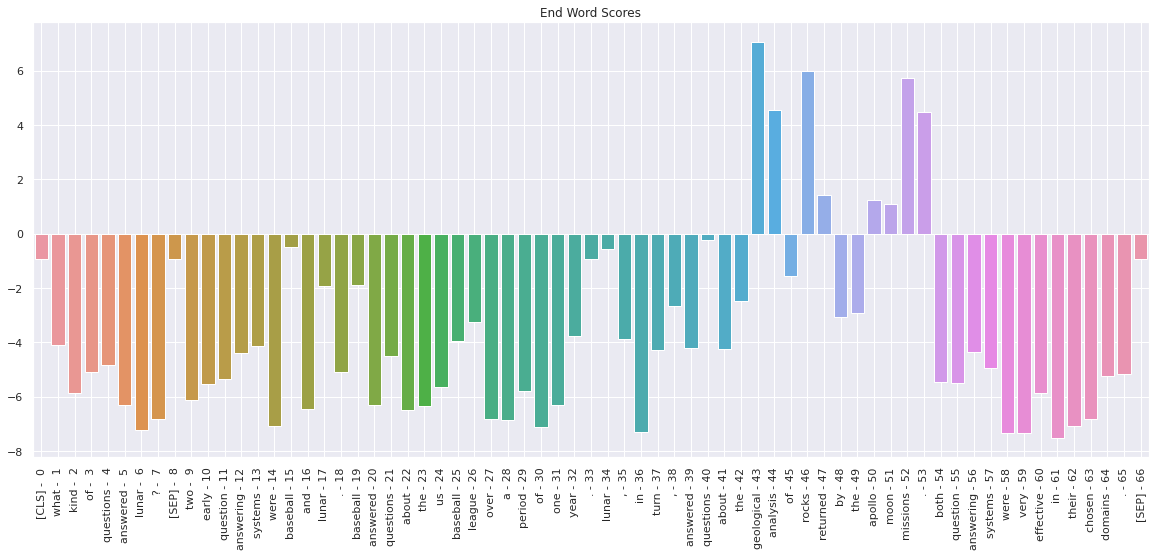
\includegraphics[width=1\linewidth]{images/end.png}
    \caption[Barplot mit der Endwortbewertung für alle Token]{Barplot mit der Endwortbewertung für alle Token}
    \label{fig:end}
\end{figure}







\clearpage
        \phantomsection % damit das pdf bookmark an die richtige Stelle zeigt
        \pdfbookmark{Literaturverzeichnis}{bibliography}
        
        % zeigt immer alle definierten Quellen an, auch wenn diese nicht verwendet werden
        %\nocite{*}
        \bibliographystyle{abbrv}
        \addcontentsline{toc}{chapter}{Literaturverzeichnis}
        \bibliography{literatur}




\chapter*{Erklärung}
Hiermit versichere ich, dass ich die vorliegende Arbeit selbstständig verfasst und keine anderen als die angegebenen Quellen und Hilfsmittel benutzt habe, insbesondere keine anderen als die angegebenen Informationen aus dem Internet. Diejenigen Paragraphen der für mich gültigen Prüfungsordnung, welche etwaige Betrugsversuche betreffen, habe ich zur Kenntnis genommen. Der Speicherung meiner Projekt-Arbeit zum Zweck der Plagiatsprüfung stimme ich zu. Ich versichere, dass die elektronische Version mit der gedruckten Version inhaltlich übereinstimmt.\newline
\linebreak
\linebreak
\linebreak
Bielefeld, den \today\newline
(Ort) (Datum)\newline
\linebreak
\linebreak
\linebreak
..................................\newline
(Unterschrift)
\end{document}